\documentclass[bibtotoc,liststotoc,BCOR=5mm,DIV=12]{scrbook}

% use this declaration to set specific page margins
\usepackage[a4paper , lmargin = {2cm} , rmargin = {4.0cm} , tmargin = {2.5cm} , bmargin = {3cm} ]{geometry}
\usepackage[a4paper]{geometry}

\usepackage[ngerman, english]{babel}
\usepackage{bibgerm}       		% german references
\usepackage[T1]{fontenc} % german characters
\usepackage{graphicx} 				% it's recommended to use PDF images but you can use JPG or PNG as well
\usepackage{url}           		% format URLs
\usepackage{hyperref} 				% create hyperlinks
\usepackage{listings, color}	% for source code
\usepackage{subfig}						% two figures next to each other (example: figure 3a), figure 3b)
\usepackage{scrlayer-scrpage}					% header and footer line
\usepackage{todonotes}
\usepackage{lipsum}     % Generate automatic filler text.


\usepackage{soul}
\usepackage[acronym,toc]{glossaries}
\usepackage{amsfonts}

\usepackage{amsmath}
\usepackage{array}
\usepackage{multirow}
\usepackage{pifont}
\usepackage{adjustbox}
\usepackage{booktabs}
\usepackage{placeins}
\definecolor{orange}{rgb}{1.0,0.55,0.0}

\setlength{\emergencystretch}{2em}
\setlength{\abovecaptionskip}{8pt plus 2pt minus 1pt}
\setlength{\belowcaptionskip}{8pt plus 2pt minus 1pt}
\setlength{\textfloatsep}{16pt plus 3pt minus 2pt}
\setlength{\floatsep}{14pt plus 3pt minus 2pt}
\setlength{\intextsep}{14pt plus 3pt minus 2pt}

\newcommand{\cmark}{\ding{51}}
\newcommand{\xmark}{\ding{55}}
\newcommand{\pmark}{\textcolor{orange}{$\sim$}}
\newcommand{\rev}[1]{\textcolor{blue}{#1}}
\newcommand{\del}[1]{\textcolor{red}{#1}}

% header and footer line - no header & footer line on pages where a new chapter starts
\pagestyle{scrheadings}
\ohead{Reasoning and Grounded Explanation Generation Using Vision--Language Models}
\ihead{Komron Valijonov}
\ofoot[]{\thepage}
\ifoot{Bachelor Thesis, UE, 2026}
\author{Komron Valijonov}

% set path where images are stored
\graphicspath{{./img/}}

\input{./misc/hyphenation} 					% use this file to set explicit hyphenations (doesn't seem to work correctly)

\makeglossaries

\begin{document}
% ---------------------------------------------------------------
\frontmatter
    \begin{titlepage}
        \centering
        \vspace*{2cm}
        {\Large Bachelor Thesis\par}
        \vspace{1.5cm}
        {\Large Reasoning and Grounded Explanation Generation Using Vision--Language Models\par}
        \vspace{2cm}
        {\Large Komron Valijonov\par}
        \vspace{0.5cm}
        {\large Department of Business, University of Europe for Applied Sciences\par}
        \vfill
        {\large First supervisor: Raja Hashim Ali\par}
        {\large Additional supervisor: Talha Ali Khan\par}
        \vspace{1cm}
        {\large 2026\par}
    \end{titlepage}

    \thispagestyle{empty}
    \cleardoublepage

    \chapter*{Statutory Declaration}
    \addcontentsline{toc}{chapter}{Statutory Declaration}
    I hereby declare that I have written this thesis independently and that I have used no sources or aids other than those indicated.
    All passages that are taken from published or unpublished sources, either literally or in substance, are marked as such.
    I also declare that this thesis has not been submitted to any other examination authority in the same or similar form.

    \vspace{2cm}
    \noindent Potsdam, 22.06.2026\hfill Komron Valijonov
    \clearpage

    \thispagestyle{empty}
    \cleardoublepage


    \chapter*{Abstract}
    \addcontentsline{toc}{chapter}{Abstract}
A vision-language model (VLM) is able to read a chart, document, scanned form, or natural image and answer questions about it. 
But how do we know if the answer is actually derived from the image itself, rather than being a lucky guess on a question based on the model's remembered language patterns?
The correctness of the answer itself is not enough if the reasoning for that answer is not grounded in the visual evidence of the image.
Charts and documents are a good example of this problem, because to answer the question correctly, the model has to actually ground its reasoning on specific parts of the image,
making it easier to spot when the model is looking at the wrong thing. Although recent work has made progress on this issue,
there was no isolation of the training objective as the main variable, with all other factors such as the model, the data, and the budget held constant.
Contrastive, generative, and explanation-based methods have all been proposed, but they have not been directly compared under the same conditions,
so it is not clear what the objective itself contributed to the final performance. 
In this paper, we keep the pipeline fixed and change only the training signal, so we can see what the objective does to answer accuracy, explanation quality, 
and evidence sensitivity when the model, the data, and the compute budget are all held steady.
We compare five settings head to head rather than treating them as unrelated systems: BLIP-2 generative fine-tuning, BLIP-2 contrastive-enhanced fine-tuning,
Qwen2-VL under answer-only, rationale-generative, and explanation-aware supervision.
All the runs use the same resource-constrained single-seed protocol, and the same evaluation code as much as possible,
across ScienceQA, A-OKVQA, ChartQA, DocVQA, and a VQAv2 subset.
The picture that emerges is mixed. On ScienceQA, Qwen2-VL-2B reaches 0.800 accuracy with answer-only supervision,
0.780 in both rationale-generative and length-aware explanation control settings, and 0.765 with fixed-alpha explanation-aware training.
On A-OKVQA, the same model reaches 0.830 with answer-only supervision, 0.790 in both rationale-generative and length-aware explanation control training,
and 0.795 with fixed-alpha explanation-aware training.
ChartQA, DocVQA, and the VQAv2 subset have no gold rationales, so those runs fall back to answer-only controls;
they lift the native headline metrics, but they do not test rationale supervision at all.
BLIP-2 barely moves: the contrastive objective gives a small gain compared to the generative one on ScienceQA 0.480 vs 0.475,
but the retrieval diagnostic stays near frozen and random controls in both cases.
Scale is the exception. With a fixed explanation-aware objective on ScienceQA, Qwen2-VL-7B reaches 0.885 while the 2B version reaches 0.765.
The masking analysis tells us whether the model relies on the image, not whether its explanation is faithful.
Overall, the results do not show a clear win for explanation-aware training.
The rationale supervision can help on a single-GPU budget, but the gain is easy to mis-credit to scale or tuning.
Hence, it only stands up when answer-only controls, objective balance, model scale, transfer and evidence sensitivity are each reported separately.

    \clearpage

    \thispagestyle{empty}
    \cleardoublepage

    \chapter*{Kurzfassung}
\addcontentsline{toc}{chapter}{Kurzfassung}
Diese Arbeit untersucht, wie unterschiedliche Trainingsziele das Verhalten von Vision--Language Models beeinflussen, wenn Modellarchitektur, Datenschema, Rechenbudget und Evaluationsprotokoll möglichst konstant gehalten werden.
Verglichen werden Zero-Shot-Referenzen, BLIP-2 mit generativer und kontrastiv-erweiterter Feinabstimmung sowie Qwen2-VL mit answer-only, rationale-generativer und explanation-aware Supervision.
Die Evaluation betrachtet nicht nur die Antwortqualität, sondern auch die Qualität generierter Begründungen und die Sensitivität gegenüber visuellen Evidenzbereichen.
Die Ergebnisse zeigen, dass explanation-aware Training in einigen Einstellungen die Begründungsqualität verbessern kann, aber nicht automatisch besser als answer-only Training ist.
Außerdem bleibt die visuelle Evidenzsensitivität getrennt von der reinen Textqualität der Begründung zu bewerten.
Die Arbeit versteht sich daher nicht als Leaderboard-Beitrag, sondern als kontrollierte Analyse von Trainingssignalen unter einem realistischen Single-GPU-Budget.

    \thispagestyle{empty}


    \tableofcontents
    \thispagestyle{empty}

    % \todo[inline]{talk to your supervisor if this is needed}
    \listoffigures
    \thispagestyle{empty}

    \listoftables
    \thispagestyle{empty}

% --------------------------------------------------------------

\mainmatter % comment single chapters for faster compilation

    \chapter{Introduction}
\section{Motivation}
Vision--language models (VLMs) are becoming a default tool for answering questions based on the content of images, documents, and charts.
The process looks simple: you give it an image and a question, and it will respond with an answer the image actually supports.
What is considered as evidence depends entirely on the picture. 
In a document it might be sitting in a line of a body text, in a table, or in a stamped region of the scanned page.
In a chart it might be in an axis label, the relative height of the bars, a colour, or a trend that is not written down explicitly in words.
In science and commonsense visual question answering (VQA), it is often not in the image at all, forcing the model to deduce the answer from the background knowledge it has already learned.
Across every one of these, a correct-looking answer is not enough if the reasoning for that answer is not actually based on what is visible in the image.
The VLMs are very good at generating the right-looking answers while looking at the wrong thing.
That is why in this paper we do not rely on the answer alone, but also check the quality of the explanation and the sensitivity of the answer to visual evidence.

The issue behind all of this is a cross-modal alignment problem: how do we connect the visual signal to the language model in a way that actually makes the two talk to each other?
It turns out that the quality of that wiring depends on many factors, such as the visual resolution, the data mixture, the connector design, the instruction tuning, and the adaptation method~\cite{laurencon2024whatmatters,zhang2025mm15,deitke2025molmo}.
Open model families are very helpful, because backbones such as Qwen2-VL, BLIP-2, and LLaVA-OneVision are strong enough out of the box, while still being adaptable on an academic budget~\cite{wang2024qwen2vl,li2023blip2,li2025llavaonevision}.
At the same time, document and chart studies show that general visual instruction following is not enough when it comes to text-heavy and structured images~\cite{fu2025textrichsurvey,wang2024docllm,masry2024chartinstruct,masry2025chartgemma}.

Furthermore, there is also a budget reality to consider.
Most students and small labs cannot afford full fine-tuning of a large multimodal model.
Methods like DoRA (weight-decomposed low-rank adaptation) make it possible to fine-tune the model by updating only a small portion of the parameters, while keeping the base model frozen or quantised~\cite{liu2024dora}.
Hence, in this study, we take the same approach using low-rank adaptation (LoRA) and its quantised variant (QLoRA) instead of full-model fine-tuning~\cite{hu2022lora,dettmers2023qlora}.
The main goal is not scoring the highest on a leaderboard, but rather to check the model's performance when only the alignment objective changes while keeping all other factors constant.

\section{Gap Analysis}
The gap is isolation.
Most papers change the model, the data, the training size, and the objective all at once.
Once the final result is reported, it is hard to tell how much the objective itself contributed.
Maybe the objective helped, but it might also be the case that it was simply a bigger model, cleaner data, or more tuning and not necessarily the objective itself.

Moreover, each objective has its own blind spot.
Contrastive learning is good at matching an image to a caption, but it does not teach the model to generate an explanation or an answer from the image.
Generative learning is good at producing an answer, but it does not necessarily mean that the model is basing its answer on the correct parts of the image.
Explanation-aware training teaches the model to actually write reasoning to come to the answer, but the model could have learned to write a convincing explanation after the fact,
which might not actually be the cause of the answer.

Hallucination and faithfulness evaluation has mostly been studied on natural images, where the common test is whether the model names objects that are not there.
Charts and documents have recently come into focus too, with benchmarks for chart hallucination, chart grounding, and document-answer groundedness emerging~\cite{wang2025charthal,bansal2025chartab,chen2025docqa}.
They are still comparatively underexplored, even though their evidence is more structured and easier to verify.
That is exactly what makes them a good test case for grounding.

These gaps are not closed by a new model or benchmark. What is actually missing is a controlled study that holds the model, the data, the budget, 
and the evaluation procedure constant while changing only the alignment objective, to test not only the answer quality but also the explanation quality and the evidence sensitivity of the model under each objective.

\section{Objective}
The goal of this thesis is to study the effect of different training objectives on vision--language model performance
while keeping all the other factors such as the model, the data, the budget, and the evaluation protocol constant.
This work is not meant to be a leaderboard submission.
Instead, it focuses on a controlled comparison where the same pipeline is used to 
study answer quality, explanation quality, and visual evidence sensitivity under a resource-constrained environment.
This enables the study to be more accessible and reproducible for students and small academic labs who may not have access to large computational resources.

The first objective is to compare different alignment strategies that are often discussed separately.
In this thesis, we place answer-only supervision, rationale-generative supervision,
explanation-aware supervision, BLIP-2 generative fine-tuning, and BLIP-2 contrastive-enhanced fine-tuning inside a single experimental frame.
This way, we achieve the comparison that focuses on the training signal rather than on uncontrolled changes in the model family, dataset pipeline, or evaluation code.

The second objective is to evaluate the answer quality and explanation quality separately.
A model can generate a correct answer without producing a strong explanation,
and it can also generate a convincing explanation without actually using the visual evidence correctly.
That is why the evaluation does not focus on a single score.
Instead, it reports the native answer metric for each dataset and also uses rationale-overlap metrics in 
the datasets where gold rationales are available, to see whether the model's explanation is actually improving in quality or just looking better on the surface.

The third objective is to check the model's sensitivity to visual evidence in the image.
We measure this with image-masking perturbations, where we compare the model's answer score before and after hiding parts of the input image.
The goal is not to prove perfect faithfulness, but to add an additional signal of evidence sensitivity alongside answer accuracy and rationale quality.

The fourth objective is to study the consistency of the same fine-tuning pipeline across different visual domains.
Therefore, we include science, commonsense, chart, document, and natural-image tasks in the study.
This matters because answering the questions in documents and charts often depends on local text, layout, labels, axes, and values,
whereas science and commonsense questions may rely more on answer choices and learned knowledge.

The fifth objective is to keep the limitations visible.
We use capped datasets, one primary seed per complete configuration, and parameter-efficient fine-tuning,
because those choices make the work feasible on a student budget, but they also define how far the claims can go.
Therefore, the results should be interpreted as controlled framework results rather than final benchmark claims.

\section{Thesis Scope}
The scope of this thesis is intentionally fixed around bachelor-level feasibility.
The study does not try to train the largest possible model or cover every possible dataset split.
It asks a narrower question: what can be learned when a practical VLM fine-tuning pipeline is kept stable and the training objective is changed?
This is why the thesis treats the capped protocol as part of the method rather than as an accidental weakness.
The cap makes the runs possible, repeatable, and easy to audit within the available time and hardware.

This also affects how the results should be judged.
A small single-seed result cannot prove that one method is universally better than another.
It can, however, show whether a proposed training signal still looks useful after answer-only controls, rationale-generative controls, masking diagnostics, and transfer checks are placed beside it.
That is the standard used here.
The thesis does not claim that explanation-aware training always wins.
It checks where it helps, where it does not help, and where the evidence is too weak to make a strong claim.

The same logic applies to the model choices.
Qwen2-VL is used for the main objective comparison because it can be adapted with QLoRA and can handle several visual domains.
BLIP-2 is used for the contrastive branch because its Q-Former gives a practical representation path for image--answer alignment.
These choices are not presented as the only valid backbones.
They are practical backbones for testing the research question under a controlled budget.

The thesis therefore sits between a small implementation project and a large benchmark paper.
It includes working code, generated artifacts, figures, tables, and a full paper-style analysis.
At the same time, it keeps the claims limited to what the completed runs can actually support.
That balance is important for this topic, because VLMs can make results look more impressive than they really are if the evaluation only reports final answer accuracy.
The central value of the work is the controlled comparison and the careful interpretation of answer quality, rationale quality, and visual sensitivity as separate outcomes.

\section{Purpose and goal}
The contribution is the controlled comparison, not a new architecture.
Instead of introducing a new architecture, we compare existing ones under different training objectives.
We consider the faithfulness of the model's reasoning as a first-class result, rather than concentrating solely on answer accuracy.
The paper contributes the following:

\begin{itemize}
    \item A comparison of zero-shot, answer-only, BLIP-2 generative, BLIP-2 contrastive-enhanced, Qwen2-VL rationale-generative, and Qwen2-VL explanation-aware alignment under the same data and optimisation settings.
    \item Evaluation along three separate axes, namely answer quality, explanation quality, and evidence sensitivity, across document, chart, science, and commonsense tasks.
    \item For multiple-choice reasoning, a generate-then-score protocol is used, so the model is evaluated only after it has produced its own reasoning trace.
    \item A direct test of how QLoRA behaves with scale, instead of assuming that full fine-tuning or very large models are the only things worth studying.
\end{itemize}

\subsection{Why this study matters}
The usefulness of this study is in the constraints.
It runs on a resource-constrained setup that is actually accessible to students and small labs.
It also avoids concentrating solely on a single aspect of performance, and instead keeps answer accuracy, explanation quality, and evidence sensitivity as separate readings.
On documents and charts especially, that separation is particularly important, because the evidence should trace back to a visible region.
The whole pipeline is reusable: every dataset is transformed into one shared format, and every experiment is declared in a configuration file,
so the code can be used for future comparisons of new objectives, new models, or new datasets, without worrying about hidden differences between runs.
And the results are honest rather than overselling: the rationale supervision does help on the science and commonsense runs, but the answer-only controls stay strong,
and the BLIP-2 contrastive objective provides only a small answer gain on top of weak retrieval evidence.

\section{Outline}
Chapter 2 provides the material needed to understand this thesis.
It includes the technical background on vision--language models, cross-modal alignment,
generative and contrastive supervision, explanation-aware learning,
parameter-efficient fine-tuning, evidence sensitivity, and the evaluation metrics used in the work.
Chapter 3 reviews the recent literature on topics such as vision--language model architectures,
document-heavy inputs, chart reasoning, faithfulness, critique, and efficient adaptation.
Chapter 4 presents the problem statement and research questions.
Chapter 5 describes the methodology used in our experiments,
including the datasets, prompt families, model setup, training objectives, evaluation protocol, and experimental settings.
Chapter 6 shows the results of the experiments and discusses their meaning in relation to the research questions, domain differences, masking analysis, model scale, and transfer behaviour.
Finally, Chapter 7 concludes the thesis and gives directions for future work.

    \chapter{Theoretical Background}
This chapter provides the technical background that is required to understand the concepts of this thesis properly.
There are many terms used in the vision--language literature that might seem similar to each other, but mean different things.
For example, answer accuracy, explanation quality, and visual grounding are related concepts, but they are measured differently.
Also, concepts like contrastive alignment, generative fine-tuning, and explanation-aware training are all about connecting the visual signal to the language model,
but they do it through different training signals and have different implications for the model's behaviour.
The main goal of this chapter is to provide enough background on these concepts so that the reader understands
what they mean, and how and why they are used in the experiments of this thesis.

\section{Vision--language models and visual question answering}
A vision--language model is a model that can process both visual and text-based inputs and produce text-based outputs.
In this thesis, the visual input can be a natural image, a chart, a scanned document, or a science-style diagram.
The text input is usually a question to be answered based on the provided image, and in some datasets it also includes answer choices.
The model is expected to generate an answer to the given question, and in some cases it is also expected to produce a rationale before answering the question.

The task throughout this thesis is visual question answering.
The structure is simple: given an image and a question as input, the model returns an answer as output.
However, the type of reasoning required to come up with the answer can be different across datasets.
In a natural-image question, the answer usually depends on recognising an object or a simple relationship between objects.
In the case of a chart question, the answer might depend on reading an axis label, comparing two bars, or estimating a value.
In a document question, the answer might be a short text region hidden somewhere inside a scanned page.
In a science or commonsense question, the model might need to combine image information with answer choices and learned background knowledge.

This variation is one of the reasons why this thesis uses multiple datasets across different domains instead of focusing on one dataset only.
A model might be good at one type of visual reasoning but perform poorly on another type of visual reasoning.
For example, a model that excels at recognising objects in natural images might still fail to read small text in a document or to compare two bars in a chart.
That is why this thesis treats visual question answering as a family of related tasks rather than one single problem.

A second important point is that the answer format is different across datasets.
In ScienceQA and A-OKVQA datasets the answers are multiple-choice, where the model does not automatically generate the answer,
but instead assigns a score to each answer choice and the highest-scoring choice is then selected as the final answer.
Other datasets, such as DocVQA, ChartQA, and VQAv2 provide open-ended or short-answer tasks, where the model produces the answer directly.
That is why the evaluation cannot use a single universal metric for every dataset and instead uses the metrics
that are native to each dataset.

The wider VQA literature shows why these task differences matter.
VQA and OK-VQA focus on natural-image and knowledge-heavy question answering,
TextVQA and OCR-VQA add text in the image,
GQA and CLEVR focus more on compositional reasoning,
and DVQA, FigureQA, PlotQA, and InfographicVQA move the same problem toward charts, plots, and infographic-style documents~\cite{agrawal2017vqa,marino2019okvqa,singh2019textvqa,mishra2019ocrvqa,hudson2019gqa,johnson2017clevr,kafle2018dvqa,kahou2018figureqa,kim2020plotqa,mathew2022infographicvqa}.


\section{Cross-modal alignment}
Cross-modal alignment means connecting signals from different modalities, such as images and language,
in a way that those modalities can interact with each other for the model to perform a certain task.
In vision--language models, the visual signal must provide useful context for the language side.
If this connection is weak, the model might still produce a convincing answer, but that answer might be coming from
the learned language patterns rather than from the visual information provided by the image.

The word alignment can mean different things in different contexts.
At the representation level, it means that the model learns that in the embedding space, the provided image and the matching text should be close to each other, while non-matching ones should be further apart.
At the generation level, it means that the model learns to use the information provided by the image when generating the output for a given task.
At the reasoning level, it means that the model learns to produce explanations that connect the question, visual input, and the final answer in a helpful way.

Earlier alignment models such as CLIP and ALIGN make the representation-level idea very clear:
matching images and text are pulled together in the embedding space,
while BLIP and Flamingo push the same alignment idea toward generation and few-shot vision--language interaction~\cite{radford2021clip,jia2021align,li2022blip,alayrac2022flamingo}.
Grounding datasets such as Visual Genome, Flickr30k Entities, ReferItGame, and RefCOCO also show the stricter version of the problem,
where the model has to connect language not only to the whole image, but also to the right region inside the image~\cite{krishna2017visualgenome,plummer2015flickr30k,kazemzadeh2014referitgame,yu2016modelingvisual}.

A model might internally have a strong text--image representation and still fail to generate a correct answer.
It might generate a correct answer without producing a useful explanation.
It might also produce a good-looking explanation that is not actually based on the right visual evidence.
That is why this thesis separates the training objective from the evaluation axis.
The training objective tells us what signal to feed the model during fine-tuning,
while the evaluation axis tells us which behaviour actually changed after fine-tuning. 

During comparison, the model design, the data handling, and the compute budget are kept constant, so that the outcome is attributed to the training objective rather than to other factors.
If one method uses a larger model, more training data, or a different prompt format, then it would be difficult to say whether the outcome is the result of the training objective or any of those other factors.
This does not make the study perfect, but it makes the comparison more focused on the effect of the training objective itself.


\section{Generative supervision}
Generative supervision is a setup in which the model is trained to produce a target token sequence.
In the answer-only case, that target sequence is comprised of the answer tokens only.
In a rationale-generative case, the target sequence contains not only the answer tokens, but also a reasoning sentence or rationale before the answer.
The model is fed an image and a question as input, and the loss is computed on the target tokens.

Since instruction-tuned VLMs already work by reading a prompt and generating text,
training them with answer/rationale text targets fits well with the way these models are used.
The model can already generate text, so fine-tuning can adapt it to produce the expected output format for a specific task.
For example, the model can learn that in ScienceQA, it should select an answer from the provided answer choices,
or that in DocVQA, it should generate a short text as the answer.
Hence, generative fine-tuning is a good baseline for many visual question answering tasks.

However, pure generative supervision has some limitations when it comes to grounding.
A model might learn to generate the answer without actually using the provided visual information correctly.
It might also just memorise common patterns in the dataset.
For example, in multiple-choice datasets, some questions could to some extent be answered by looking at the question and the answer choices alone,
without actually looking at the image.
In documents and charts, the model could memorise that the answer is often in some specific position or format.
This does not mean that generative supervision is not a good option, but it does mean that in the evaluation phase, we need to check more than just the final answer accuracy
to make sure that the model is actually using the visual signal in a meaningful way.

In this thesis, we use generative supervision in two ways.
First, we use it as a direct training objective for the BLIP-2 and Qwen2-VL runs that are not explanation-aware.
Second, we use it as a control for the explanation-aware training.
This is quite important, because we do not want to compare the explanation-aware supervision only against a frozen zero-shot model,
but also against pure generative supervision that was fine-tuned to produce the expected answer or rationale-plus-answer text without
the same span-weighting strategy. 


\section{Contrastive supervision}
Contrastive supervision is a way to train the model to bring the image and text representations closer to each other when they match,
and to push them apart when they do not match.
In this thesis, we use contrastive supervision as an additional signal on top of generative fine-tuning, not as a replacement for it.
We still train the model to generate the answer, but in addition to that, we also give it a contrastive signal over image--answer representations.
We use BLIP-2 for this setup, because it has a Q-Former that uses a fixed number of learnable query tokens to pool visual information from the image encoder outputs, which can then be used to build an image representation.
The basic idea is that the image representation should be closer to the correct answer representation than to other answers in the same batch.

This contrastive-enhanced setup is different from ordinary text generation.
The generative part asks the model to generate the next target token.
The contrastive part asks the model to organise the image and answer representations in such a way that the correct image--answer pair is easier to retrieve than mismatched pairs.

In principle, this can encourage the model to learn stronger image--answer alignment.
In practice, however, the effect of the contrastive signal depends on many factors, such as the model architecture, the way the image representation is extracted,
the design of the projection head for contrastive learning, the batch size used during training, and the nature of the data.
Hence, we do not assume that the contrastive branch is useful just because it adds an additional loss term.
Instead, we test the contrastive-enhanced setup directly against a BLIP-2 generative fine-tuning control, to check whether it actually leads to better results.

One of the important things to check is the retrieval diagnostic.
If the contrastive supervision is doing what we expect, the correct answer should be easier to retrieve from the image representation than mismatched answers.
A simple way to check that is to compute Recall@1, Recall@5, Recall@10, and mean reciprocal rank.
These metrics do not directly measure the final answer accuracy, but they give us a way to see if the contrastive objective is actually adding any value in terms of representation alignment.

A modest contrastive result does not mean that contrastive supervision is useless in general.
It only means that under our specific setup, with the chosen BLIP-2 configuration and the capped ScienceQA run, the contrastive-enhanced fine-tuning
does not lead to a better result than the generative fine-tuning control.
This is important to note, because the thesis is about the controlled effect of the training objective under the available budget, not about dismissing an entire class of methods.


\section{Rationales and explanation-aware learning}
A rationale is a text generated before the final answer that explains how to connect the question and the visual input to come up with the answer.
Not all the datasets provide gold rationales.
Hence, for the rationale supervision, we use only the datasets that provide gold rationales, which are ScienceQA and A-OKVQA.
With those runs, we can check whether rationale supervision improves answer accuracy and explanation quality.

Explanation-aware supervision is very similar to rationale supervision with the only difference in the training loss.
In rationale supervision, we train the model to generate a rationale and an answer in one sequence, and the loss is computed over the entire sequence.
In explanation-aware supervision, we split the target into two spans: the explanation span and the answer span.
The training loss is then computed separately for each span, and a coefficient $\alpha$ is used to weight the answer loss compared with the explanation loss.
This allows us to test whether answer supervision and rationale supervision help each other or compete with each other.

There is an ablation sweep done over $\alpha$ to check how the balance between answer and explanation supervision affects the results.
When $\alpha$ is low, the model receives more signal from the explanation span,
which encourages it to produce better rationales, but it might not focus enough on getting the answer right.
On the other hand, when $\alpha$ is high, the model receives more signal from the answer span,
which encourages it to produce better answers, but it might not focus enough on producing good rationales.
The third setting is a length-aware control,
where $\alpha$ is set based on the number of tokens in the explanation and answer spans.
This control is useful because fixed $\alpha$ values might give a misleading impression of what explanation-aware training is doing.

A key limitation is that only datasets with gold rationales can directly support rationale-supervised training.
ScienceQA and A-OKVQA provide this supervision in the completed experiments.
ChartQA, DocVQA, and VQAv2 do not provide the same type of gold rationale in this setup.
For those datasets, the thesis uses answer-only fallback training and transfer testing instead of treating them as explanation-aware datasets.
This is why the interpretation of results changes by domain.

Rationale quality is also not the same as faithfulness.
A generated explanation can overlap with the gold rationale and still fail to prove that the model actually used the image.
For example, the model might learn a common explanation pattern from training data.
It might also generate a reasonable explanation after choosing the answer for some other reason.
This is why rationale metrics are reported beside, not instead of, evidence-sensitivity analysis.

\section{Parameter-efficient fine-tuning}
Full fine-tuning updates all or most of the parameters in a model.
For large vision--language models, this can be expensive in memory, compute, and time.
Parameter-efficient fine-tuning updates only a small number of additional parameters while leaving most of the base model frozen or quantised.
This makes experiments possible on a much smaller budget.

LoRA is one common parameter-efficient method.
Instead of updating a full weight matrix directly, LoRA adds low-rank trainable matrices that modify the behaviour of selected layers.
QLoRA extends the idea by loading the base model in quantised precision and training low-rank adapters on top of it.
This makes the memory requirement lower while still allowing the model to adapt to the task.
In this thesis, Qwen2-VL runs use QLoRA so that both the broad sweep and the 7B scale check can fit the available environment.

LoRA and QLoRA are part of a larger family of parameter-efficient methods.
Adapters, prefix tuning, prompt tuning, P-tuning v2, BitFit, and vision--language adapters all follow the same practical direction:
change a small trainable part of the model instead of updating the whole backbone~\cite{houlsby2019adapters,li2021prefix,lester2021prompt,liu2022ptuningv2,zaken2022bitfit,sung2022vladapter}.

Parameter-efficient fine-tuning is not only a practical trick.
It also shapes the research question.
The thesis asks what can be learned under a resource-constrained setup, not what could be achieved with unlimited compute and full-model fine-tuning.
That is why the results should be read as fixed-budget comparisons.
A method that works well under these constraints is useful for students, small labs, and early-stage research projects.
A method that only works after very large compute investment would answer a different question.

Using QLoRA also makes the scale comparison more controlled.
The 2B and 7B Qwen2-VL runs are not compared by changing the whole training strategy.
Both use the same explanation-aware setting and the same parameter-efficient adaptation style.
This makes the observed difference more about backbone scale than about changing the fine-tuning method.
The comparison is still not a full efficiency benchmark because exact runtime and peak memory are not measured as primary results.

\section{Evidence sensitivity and masking}
Evidence sensitivity asks whether the model's answer changes when relevant visual information is removed or altered.
In this thesis, the diagnostic is based on masking regions of the image.
The model is scored on the full image, then scored again after a region is hidden.
If the score for the correct answer drops after masking, the model was sensitive to that region.

This is related to the broader explainability literature.
Methods such as Grad-CAM, LIME, Integrated Gradients, and Transformer attribution also try to connect model behaviour back to input evidence,
but this thesis uses a simpler score-change masking diagnostic instead of claiming a full causal explanation~\cite{selvaraju2017gradcam,ribeiro2016lime,sundararajan2017axiomatic,chefer2021transformer}.

This is a useful diagnostic, but it must be interpreted carefully.
A high drift value means the answer score depends on the masked region.
It does not automatically prove that the generated rationale is faithful.
A model may rely on a visual region without describing it correctly.
It may also produce a good-looking rationale while the answer score barely changes when the image is masked.
For that reason, masking drift is treated as evidence sensitivity rather than a full proof of faithful explanation generation.

Masking is also affected by the domain.
In documents and charts, evidence can be local: a number in a table, a word in a scanned form, an axis label, or a bar height.
Masking such a region can strongly change the answer score.
In science and commonsense images, the evidence may be more diffuse, or the answer may be partly recoverable from the question and answer choices.
In that case, masking one coarse region may produce a smaller drift even when the image still matters.

The thesis therefore uses masking as one part of the evaluation, not as the only faithfulness measure.
It is strongest when read together with answer accuracy, rationale metrics, and qualitative examples.
The qualitative masking figure is included to show what kind of visual perturbation was applied and how the scores changed.
It is not meant to replace a human annotation study of faithful reasoning.

\section{Metrics used in the thesis}
The datasets in this thesis use different native metrics, so the results are not read as one universal score.
ScienceQA and A-OKVQA use multiple-choice accuracy in the main experiments.
ChartQA uses relaxed accuracy because numerical answers can have small acceptable differences.
DocVQA uses average normalised Levenshtein similarity, which gives partial credit for short text answers that are close to the target.
The VQAv2 subset uses VQA consensus accuracy where annotator answers are available.

The term headline metric refers to the main metric for a dataset.
It does not mean that a score on one dataset can be directly compared with a score on another dataset.
For example, 0.80 multiple-choice accuracy on ScienceQA and 0.80 ANLS on DocVQA do not mean the same thing.
They are both strong within their own benchmark context, but they measure different answer formats.
This is why the thesis compares models mostly within a dataset or within a clearly stated transfer column.

BLEU and ROUGE-L are used only when gold rationales are available.
They measure overlap between generated text and reference rationale text.
They are useful because they provide a repeatable automatic check, but they are limited.
A correct explanation can use different wording and receive a lower overlap score.
A high-overlap explanation can still fail to prove visual grounding.
For this reason, the thesis describes them as rationale quality metrics, not as complete faithfulness metrics.

Other text-quality metrics such as METEOR, BERTScore, and BLEURT are also common in generation evaluation,
especially when exact lexical overlap is too narrow.
They are not used as primary results here, because the goal is to keep the rationale-quality analysis lightweight and repeatable under the same fixed pipeline~\cite{banerjee2005meteor,zhang2020bertscore,sellam2020bleurt}.

The uncertainty intervals are also used cautiously.
Most completed evaluation sets are capped, and the main configurations use one seed.
Small differences such as 0.790 versus 0.795 should therefore be read as observed single-run differences.
They are not treated as conclusive evidence that one method is definitely better.
This is especially important in the BLIP-2 comparison and the A-OKVQA explanation-aware comparison, where the numerical gaps are small.

\section{Prompt families and model-facing text}
The prompt family is part of the experiment, not a small implementation detail.
If two models are trained or evaluated with different prompt styles, then a difference in performance may come from the prompt rather than from the training objective.
For that reason, this thesis separates answer-only prompts from rationale prompts and keeps this choice visible in the experiment ledger.
An answer-only run receives a question and is trained to produce only the final answer.
A rationale-generative or explanation-aware run receives the same visual question, but the target text contains a reasoning part before the final answer.

This distinction matters most for datasets with gold rationales.
ScienceQA and A-OKVQA can support rationale-supervised training because the dataset already contains explanations.
For those datasets, the model can be asked to produce a short reasoning trace and then the answer.
For ChartQA, DocVQA, and VQAv2, the completed setup does not have gold rationale labels.
Using rationale targets there would require an extra annotation or teacher-generation step, which would introduce a different source of supervision.
Therefore, those datasets are treated as answer-only in-domain and transfer settings.

The model-facing text is not exactly the same as the human-readable prompt written in the paper.
The processor inserts special tokens, image placeholders, and model-specific chat formatting.
This means that the actual tensor seen by the model is longer and more structured than the plain question shown in the dataset table.
The pipeline therefore saves sample traces that show the raw example, the rendered prompt, the target, the decoded token sequence, and the supervised spans.
Those traces are included as artifacts because they make the training process inspectable instead of hidden inside the collator.

This is also why the thesis avoids describing a run only as ``fine-tuned''.
Fine-tuning can mean different things depending on the prompt and target.
An answer-only adapter is trained on a different target than a rationale-generative adapter.
An explanation-aware adapter uses the same rationale-plus-answer target family, but it applies different loss weights to the answer and explanation spans.
So, when results are compared, the comparison has to say which prompt family and which target family were used.

\section{Collation and supervised spans}
Collation is the step where raw examples become tensors.
For this thesis, the raw example contains an image, a question, optional answer choices, a gold answer, and sometimes a gold rationale.
The collator turns that example into model inputs such as token IDs, attention masks, image tensors, and labels.
The labels tell the model which tokens should receive loss.
Prompt tokens are usually masked out, because the model should not be trained to reproduce the question.
Target tokens remain supervised, because they are the text the model is supposed to learn to generate.

This step is easy to underestimate.
In a normal text-only model, one might count the prompt length using a tokenizer and then start the labels after that point.
In a multimodal model, the processor may add image tokens before or inside the text representation.
If the label mask is shifted by even a few tokens, the model can be trained on the wrong span without an obvious runtime error.
The pipeline avoids this by measuring the prompt and full sequence through the same multimodal processor.
That makes the supervised answer and rationale spans line up with the sequence that is actually given to the model.

The span information is used by more than one objective.
For ordinary answer-only training, the supervised span is the answer target.
For rationale-generative training, the supervised span covers the rationale and answer target together.
For explanation-aware training, the rationale and answer spans are tracked separately so that the loss can weight them with alpha.
For the BLIP-2 contrastive-enhanced run, only the answer span is pooled into the contrastive text representation, while the rationale span still receives generative loss where it exists.
This keeps the contrastive signal focused on matching the image to the answer rather than to a longer explanation paragraph.

The saved sample traces are therefore not just debugging output.
They are part of the research record.
They show whether the answer-only run really excludes the rationale from the target.
They show whether the explanation-aware run actually has separate explanation and answer spans.
They also show whether decoded tokens match the intended prompt and target format.
Without this audit, a result could look mathematically valid while being based on the wrong supervision.

\section{Transfer evaluation}
Transfer evaluation asks what happens when an adapter trained in one source setting is evaluated on another target dataset or prompt family.
This is different from in-domain adaptation.
In-domain adaptation asks whether a model improves on the same dataset family it was trained on.
Transfer asks whether the learned behaviour carries over when the visual format, answer style, or prompt family changes.
For this thesis, that distinction is important because the domains are deliberately different.
Science questions, commonsense images, charts, documents, and general natural images do not stress the model in the same way.

The transfer matrix should not be read as a claim that one dataset is universally easier than another.
Each column uses the metric appropriate for that target dataset, and each source adapter may have learned a different output style.
For example, a ScienceQA rationale model may learn to produce reasoning before choosing an option, while a DocVQA answer-only model may learn short extractive text answering.
When these adapters are moved across domains, the result depends on both the learned objective and the target prompt.
This is why the transfer result is discussed as a pattern, not as a single ranking.

The most useful part of transfer evaluation is that it exposes when a gain is narrow.
A model can improve strongly in-domain but transfer poorly because it has adapted to the source dataset format.
Another model can have a smaller in-domain gain but transfer better to related visual formats.
For example, document and chart tasks can share some text-heavy or layout-heavy behaviour even though the images look different.
This kind of result helps prevent the thesis from treating a single benchmark as the whole story.

The transfer setting also explains why no-rationale datasets still matter.
ChartQA, DocVQA, and VQAv2 do not support rationale-supervised training in the completed setup, but they still test whether the same fine-tuning framework works outside rationale-heavy science and commonsense tasks.
They also give target domains for transfer analysis.
So those datasets are not unnecessary; they answer a different part of the thesis.
They show where answer-only adaptation and source-trained adapters work or fail when the visual domain changes.

\section{Reproducibility and artifact record}
Because the experiments are capped and single-seed, the artifact record is important.
The thesis cannot rely on the claim that results are obvious from large-scale repeated runs.
Instead, every completed run has to be traceable: which configuration was used, which dataset split was selected, which checkpoint was evaluated, which metric was computed, and which table or figure used the result.
This is why the pipeline writes an experiment ledger, a split audit, result tables, generated figures, and a claim-to-evidence map.

The experiment ledger records the backbone, dataset, objective, train and evaluation caps, prompt family, rationale availability, and primary metric.
This makes the comparison readable before the results are shown.
The split audit records the selected source split and checks whether selected training and evaluation identifiers overlap where native identifiers are available.
The purpose is to avoid accidental leakage and to make the capped protocol honest.
If a dataset source exposes only validation and test splits, the pipeline records exactly how the controlled split was built.

The claim-to-evidence map serves a different purpose.
It links each important claim in the abstract, highlights, discussion, and conclusion to a result row, table, figure, or artifact.
This is useful because it stops the paper from making a broader claim than the results support.
For example, a masking result can support a statement about evidence sensitivity, but it cannot by itself prove faithful explanation generation.
Likewise, a DocVQA answer-only result can support a claim about capped document answering, but it cannot support a claim about document rationale faithfulness.

The final validation step checks for missing expected runs, stale results, failed runs, and missing artifacts.
This does not make the experiments statistically stronger, but it makes the reporting cleaner.
It reduces the chance that a table is built from an old configuration or that a figure silently disappears after a partial run.
For a small thesis project, this kind of bookkeeping is part of research quality.
It keeps the scope modest, but it makes the completed scope easier to defend.

    \chapter{Related Work}
The review covers relatively latest works in the areas of vision--language model design,
text-rich and document-heavy images, charts and structured visual reasoning, faithfulness and critique, and efficient adaptation.
We group it by the parts that actually matter here the most: model design, text-rich images, chart reasoning, faithfulness, datasets, metrics, and low-budget adaptation.

\section{Recent vision--language model design}
Recent vision--language models are not built around a single alignment trick.
Their performance is a result of many choices working together, such as the backbone architecture,
the visual tokenisation method, the data mixture, the connector design, and the instruction tuning.
Since all those factors are usually changed together, it is hard to tell which part actually caused an improvement in the final performance.

This is exactly the issue raised by recent ablation studies, 
which demonstrate that these factors are still poorly separated, and that it is vital to conduct controlled comparisons~\cite{laurencon2024whatmatters}.
MM1.5 also makes the same argument, showing that optical character recognition (OCR) data,
synthetic captions, instruction mixtures, and specialised variants 
can each weigh as much as raw scale in the final performance of a vision--language model~\cite{zhang2025mm15}.
Molmo and PixMo are useful here because they provide open weights and open data 
that let us actually read the recipe and understand what is going on under the hood~\cite{deitke2025molmo}.
LLaVA-OneVision shows that a single family of models can be used across image and video when the data mixture is chosen with care~\cite{li2025llavaonevision}.
The same development can also be seen in earlier and related open VLM families.
OFA and GIT frame visual tasks as generation problems,
while Qwen-VL, PaLI, OpenFlamingo, CogVLM, LLaVA, MiniGPT-4, and InstructBLIP show different ways of connecting a visual encoder with a language model and instruction-tuning it for practical use~\cite{wang2022ofa,wang2022git,bai2023qwenvl,chen2023pali,awadalla2023openflamingo,wang2024cogvlm,liu2023llava,zhu2023minigpt4,dai2023instructblip}.

For this study, the conclusion is simple.
If the model, the data, and the budget are all changing together, then the contribution of the objective itself is hard to tell.
That is why we need a controlled comparison, where the model, the data, and the budget are held constant while only the training signal changes.

Open model families are also important, because they enable us to actually run the controlled comparison on a practical budget.
Qwen2-VL is designed to work with dynamic image resolution and text-heavy visual inputs such as documents, charts, and diagrams~\cite{wang2024qwen2vl}.
BLIP-2's Q-Former lets us test an image--answer contrastive loss while keeping the larger vision encoder and language model frozen~\cite{li2023blip2}.
We use these open models because they make controlled, parameter-efficient experiments feasible under limited resources.

\section{Text-rich and document-heavy images}
Documents are difficult for a specific reason.
The answer in this case is not in the whole image, but rather in a small part of it, such as a line of text, a table cell, or a layout region.
Hence, the task is not just an image recognition problem.
The model has to read the document and find the evidence in the right place, which is a different skill than naming objects in a natural image.

Recent work shows that text-rich image reasoning is moving toward multimodal large language models, especially for OCR-heavy and layout-heavy inputs~\cite{fu2025textrichsurvey}.
DocLLM is a good example of this trend. It encodes the document layout directly into the generative document-understanding problem,
which is a step toward more faithful reasoning on documents~\cite{wang2024docllm}.
OmniDocBench focuses on the coverage angle instead, scoring diverse PDF parsing cases with detailed annotations,
which is a step toward more structured evaluation of document understanding~\cite{ouyang2025omnidocbench}.
In this study, we use DocVQA as a test case for document understanding, because it is a well-known benchmark 
where the answer is usually located on scanned text, layout, and local visual context~\cite{mathew2021docvqa}.

Our goal is not to build a new document model.
We want to see how much the training objective itself contributes to the model's ability to read documents and answer questions about them.

\section{Charts and structured visual reasoning}
Charts create a different kind of problem.
In this case, the model has to read the labels, understand the axes and tick marks,
and determine the relationships between the visual elements, such as bars, lines, or points.
ChartInstruct and ChartGemma demonstrate that instruction tuning on chart images can help in both chart understanding and reasoning~\cite{masry2024chartinstruct,masry2025chartgemma}.
ChartMimic shows the same point by training a model to generate code for that chart, which makes the model understand the chart in a more structured way~\cite{yang2025chartmimic}.
ChartMuseum shows that current large visual--language models still perform far poorer than humans on chart reasoning~\cite{tang2025chartmuseum}.
MathVista, MMMU-Pro, and MMReason extend this concern to mathematical and multi-step reasoning, which is often required for chart understanding~\cite{lu2024mathvista,yue2025mmmupro,yao2025mmreason}.

This is why we use ChartQA, ScienceQA, and A-OKVQA in the same study~\cite{masry2022chartqa,lu2022scienceqa,schwenk2022aokvqa}.
Together, they cover structured chart reasoning, science reasoning, and knowledge-heavy visual reasoning.


\section{Faithfulness, critique, and efficient adaptation}
Explanation-aware training has a subtle problem.
The model might learn to write an explanation that looks convincing,
but that is not actually based on the image and is not the real cause leading to the answer.
Recent studies approach this problem from different angles.
MMMU tests expert-level multimodal reasoning across many visual formats, to see if VLMs can do expert-style visual reasoning and not just simple image captioning~\cite{yue2024mmmu}.
MMStar checks whether a model actually needs the image to answer the question or whether the answer can be derived from the learned knowledge alone~\cite{chen2024mmstar}.
HallusionBench focuses on cases where language hallucination and visual illusion appear together in LVLM responses~\cite{guan2024hallusionbench}.
Hallucination-augmented contrastive learning turns a hallucination into a contrastive signal, to teach the model to avoid it~\cite{jiang2024hacl}.
VISCO and Critic-V evaluate the model's ability to critique, correct, and detect errors in its own output~\cite{wu2025visco,zhang2025criticv}.
General multimodal benchmarks such as POPE, MME, MMBench, SEED-Bench, and MM-Vet are also relevant here,
because they test hallucination, perception, reasoning, and instruction-following outside one narrow dataset score~\cite{li2023pope,fu2023mme,liu2023mmbench,li2024seedbench,yu2024mmvet}.
These works suggest that faithfulness should be measured separately from answer accuracy.

Efficient adaptation is also important,
because it allows us to test the effect of the training objective without needing to fine-tune the entire model.
DoRA is a good example of this approach, which demonstrates that we can actually adapt the model by updating only a small portion of the parameters~\cite{liu2024dora}.
Reason-RFT points to another direction that is relevant here, where post-training specifically rewards visual reasoning~\cite{tan2025reasonrft}.
In this paper, we stay with supervised objective comparisons, but the concern is similar.
We evaluate the model as a reasoning system, rather than only as an answer generator.

Table~\ref{tab:LiteratureSummary} summarises the relevant works and the gaps we address in this study.
It is not meant to be a comprehensive review of the field, but rather a snapshot of the recent trends and how they relate to our controlled comparison.

\begin{table*}[!ht]
\centering
\caption{Representative related work and how it connects to the gap studied here. A check mark means the line of work directly covers the property, a cross means it is not part of the main scope, and a tilde means partial coverage.}
\label{tab:LiteratureSummary}
\scriptsize
\begin{adjustbox}{max width=\textwidth}
\begin{tabular}{|p{3.2cm}|p{2.4cm}|c|c|c|c|p{4.5cm}|}
\hline
\textbf{Work} & \textbf{Main focus} & \textbf{Generation} & \textbf{Structured VQA} & \textbf{Rationales} & \textbf{Efficient FT} & \textbf{Connection to this study} \\ \hline
Recent VLM construction~\cite{laurencon2024whatmatters,deitke2025molmo,li2025llavaonevision,zhang2025mm15} & Model and data recipe & \cmark & \pmark & \pmark & \pmark & Shows that model design and training data must be controlled before we can attribute gains to the objective. \\ \hline
Open VLM backbones~\cite{wang2024qwen2vl,li2023blip2} & Adaptable model families & \cmark & \pmark & \pmark & \pmark & Provide practical backbones for controlled experiments under a fixed compute budget. \\ \hline
Text-rich document work~\cite{fu2025textrichsurvey,wang2024docllm,ouyang2025omnidocbench} & Documents and PDF parsing & \cmark & \cmark & \pmark & \pmark & Motivates the document setting, but usually does not compare training objectives under one fixed backbone. \\ \hline
Chart reasoning work~\cite{masry2024chartinstruct,masry2025chartgemma,tang2025chartmuseum,yang2025chartmimic} & Chart understanding & \cmark & \cmark & \pmark & \pmark & Shows that chart reasoning is still difficult and needs structured evaluation beyond ordinary image QA. \\ \hline
Recent reasoning benchmarks~\cite{lu2024mathvista,yue2024mmmu,chen2024mmstar,yue2025mmmupro,yao2025mmreason} & Harder multimodal evaluation & \pmark & \cmark & \pmark & \xmark & Motivate evaluation on visual, mathematical, expert-level, and multi-step reasoning tasks. \\ \hline
Faithfulness and critique~\cite{guan2024hallusionbench,jiang2024hacl,wu2025visco,zhang2025criticv} & Reliability of reasoning & \pmark & \cmark & \cmark & \xmark & Support the need to measure hallucination, critique, and evidence use separately from answer accuracy. \\ \hline
DoRA / Reason-RFT~\cite{liu2024dora,tan2025reasonrft} & Efficient and reasoning-focused adaptation & \pmark & \xmark & \pmark & \cmark & Motivate low-resource adaptation and explicit reasoning-oriented post-training. \\ \hline
This study & Controlled explanation-aware alignment & \cmark & \cmark & \cmark & \cmark & Compares objective choices directly and reports answer accuracy, rationale quality, and evidence sensitivity together. \\ \hline
\end{tabular}
\end{adjustbox}
\end{table*}

A common pattern emerges from this review.
Earlier work on multimodal alignment focused mainly on learning image--text representations, or on generating an answer from the image and the question.
More recent work has started to pay attention to the faithfulness of the model's reasoning, and to the quality of the explanations it generates.
However, it is still unclear how much the training objective itself contributes to the model's performance.
In this study, our goal is to fill that gap by conducting a controlled comparison of different training objectives while keeping all other factors constant.

    \chapter{Research Question}
\section{Problem Statement}
The problem is cross-modal alignment in a resource-constrained environment.
Given the same pretrained vision--language model, we analyse the effect of different training objectives on answer accuracy, explanation quality, and evidence sensitivity.
The model, the data format, the optimiser, and the evaluation process are kept constant wherever possible, leaving only the training signal as the variable.
The BLIP-2 pair reuses one Q-Former training setup. The Qwen2-VL generative and explanation-aware runs reuse one QLoRA setup.
The goal is not to find the best scoring setup, but to observe whether the chosen objective leads the model in a direction that matters for a more trustworthy reasoning,
and to check whether the answer quality, the explanation quality, and the evidence sensitivity move together or separately under each objective.

\section{Research Questions}
The main question is to investigate how the resource-constrained vision--language model should be aligned to achieve both accurate and faithful visual reasoning.
The following research questions break that down into more measurable parts.

\begin{enumerate}
    \item RQ1: How have vision--language alignment methods evolved for grounded visual reasoning and explanation generation?
    \item RQ2: How does BLIP-2 generative fine-tuning compare with BLIP-2 contrastive-enhanced fine-tuning on visual reasoning?
    \item RQ3: Does explanation-aware fine-tuning improve answer accuracy and explanation quality on datasets with gold rationales?
    \item RQ4: How does the same fine-tuning framework perform across document, chart, science, commonsense, and natural-image domains?
    \item RQ5: How sensitive are the model's answers to visual evidence under image-masking perturbations?
    \item RQ6: How does the selected explanation-aware QLoRA setup scale from Qwen2-VL-2B to Qwen2-VL-7B?
    \item RQ7: How well do fine-tuned adapters transfer across visual domains and prompt formats?
\end{enumerate}

    \chapter{Methods}
The main rule in this methodology is to keep the pipeline unchanged and modify only the training objective.
Each dataset is transformed into a uniform format.
Then, the model is loaded, QLoRA adapters are applied if needed, the model is trained with the chosen objective,
and evaluation is performed using the same generate-then-score protocol for every run.
Figure~\ref{Fig:Figure1} shows the full pipeline.

We intentionally keep the pipeline simple and controlled, because the goal is to isolate the effect of the training objective,
not to find the best possible score on each dataset.
Every experiment is defined through a configuration file that declares the dataset, the backbone, the objective, the adapter settings, the metrics, and the seed.
The same implementation is used for baseline evaluation, fine-tuning, and final evaluation, reducing the risk of hidden differences affecting the results.

\begin{figure}[!t]
\centering
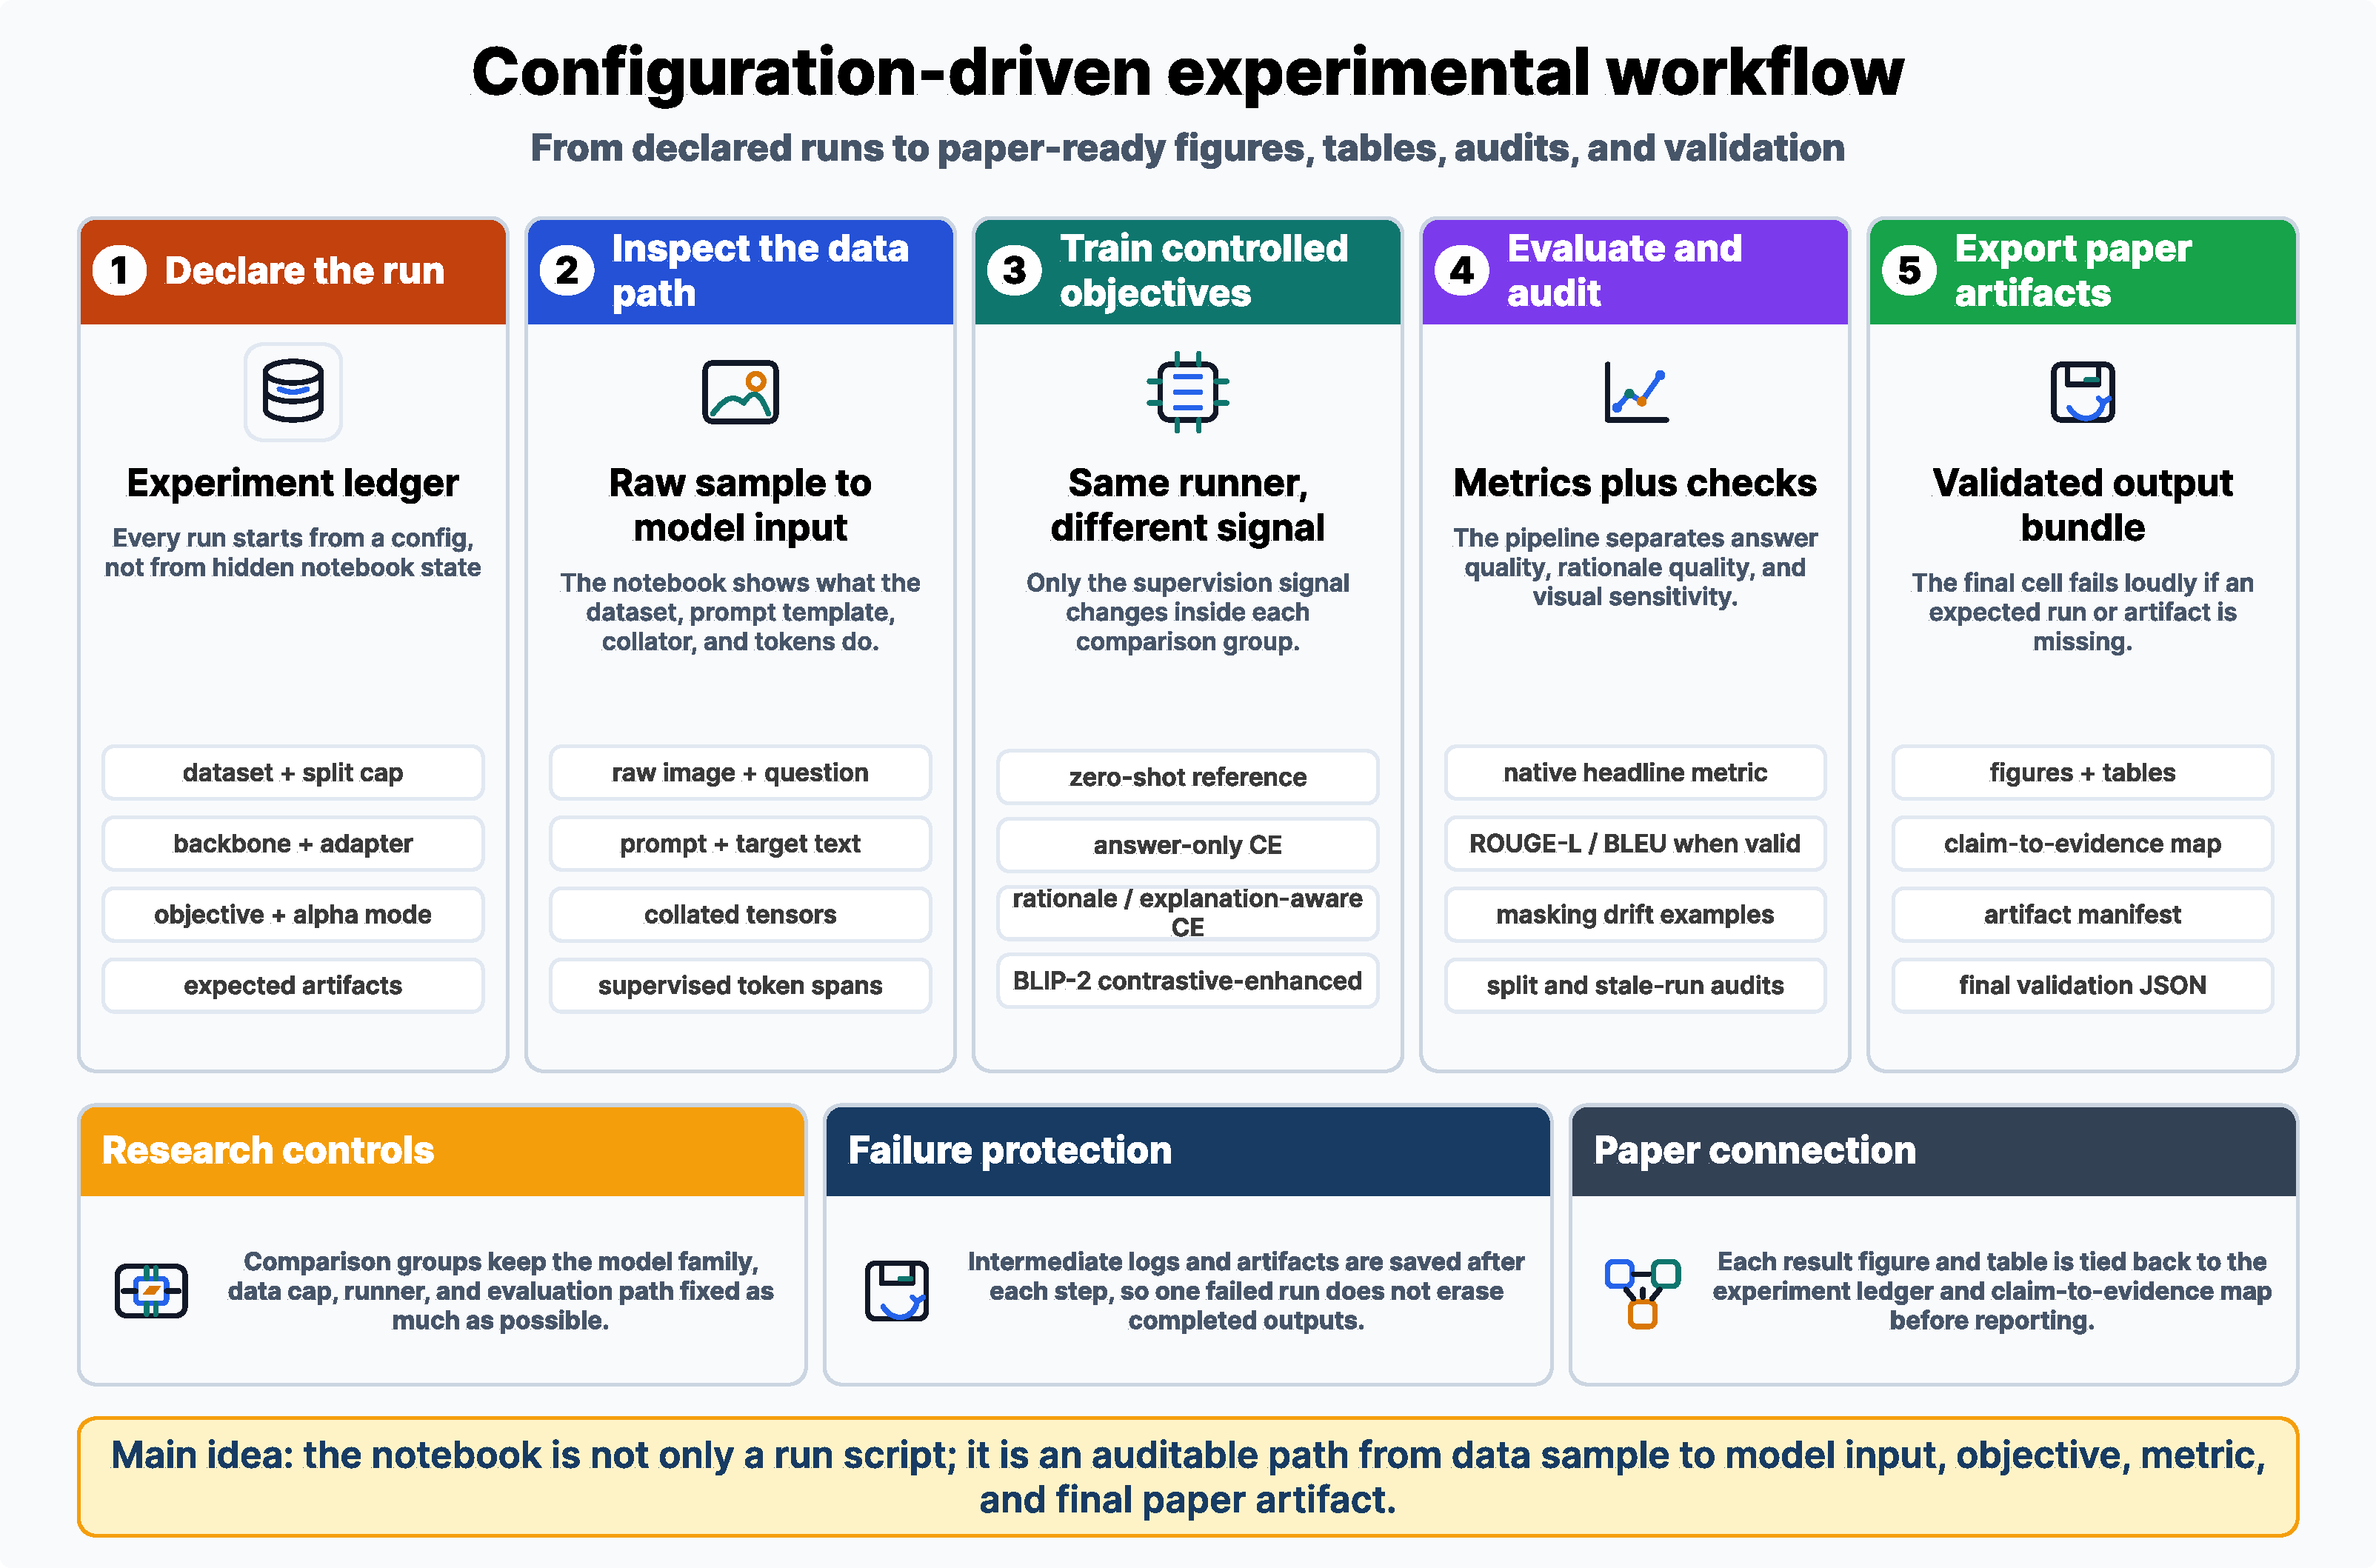
\includegraphics[width=1\linewidth]{./Figures/icons/Pipeline}
\caption{Configuration-driven experimental workflow.
Each run is declared through an experiment ledger, inspected through the data and prompt path, trained under the selected objective, evaluated with answer, rationale, and visual-sensitivity checks, and exported as paper-ready figures, tables, logs, and validation artifacts.}
\label{Fig:Figure1}
\end{figure}

\section{Datasets}
The experiments use five public datasets.
DocVQA represents document understanding, where the answer is usually based on scanned text, layout and local regions of the image~\cite{mathew2021docvqa}.
ChartQA is used for chart reasoning, in which the answer might depend on labels, axes, values, or relationships between elements in the chart~\cite{masry2022chartqa}.
ScienceQA provides multimodal science questions with multiple-choice answers and explanations, which is used for rationale supervision~\cite{lu2022scienceqa}.
A-OKVQA adds commonsense questions and rationales over natural images, which is also used for rationale-supervised training~\cite{schwenk2022aokvqa}.
VQAv2 is used as a general natural-image control, where the answer is often based on object recognition and simple relationships in the image~\cite{goyal2017vqav2}.
Table~\ref{tab:Datasets} summarises this dataset setup.

There is one important detail about the VQAv2 subset.
The experiment uses the configured \texttt{Erland/VQAv2-sample} source, which has 900 training examples and 100 evaluation examples.
Hence, we report it as a VQAv2 subset result, not as a full VQAv2 benchmark score.

All the datasets are transformed into a uniform format, where each example is comprised of an image, a question, an answer, and optionally a rationale.
If the dataset does not have gold rationales, the rationale field is left empty, and the training falls back to answer-only supervision.
Table~\ref{tab:InputConstruction} shows how these fields are turned into prompts and supervised targets.


\begin{table}[!ht]
\centering
\caption{Benchmarks used in the study. The sizes are rounded public benchmark sizes before filtering by image availability, answer type, or rationale availability. The completed experiments use capped train and evaluation splits so that every run fits the same practical compute budget.}
\label{tab:Datasets}
\begin{adjustbox}{max width=\textwidth}
\begin{tabular}{|l|l|c|l|c|l|}
\hline
\textbf{Dataset} & \textbf{Domain} & \textbf{Approx.\ size} & \textbf{Answer type} & \textbf{Gold rationale} & \textbf{Primary metric} \\ \hline
DocVQA~\cite{mathew2021docvqa} & Document & 50K & short text span & no & ANLS \\
ChartQA~\cite{masry2022chartqa} & Chart & 32K & numeric / short text & no & relaxed accuracy \\
ScienceQA~\cite{lu2022scienceqa} & Science image & 21K & multiple choice & yes & accuracy \\
A-OKVQA~\cite{schwenk2022aokvqa} & Commonsense image & 25K & multiple choice / short text & yes & accuracy \\
VQAv2 subset~\cite{goyal2017vqav2} & Natural image & 900/100 run split & open ended & no & VQA accuracy \\ \hline
\end{tabular}
\end{adjustbox}
\end{table}

\begin{table*}[!ht]
\centering
\caption{Input construction examples. The complete token, label, span, and collator traces are saved as pipeline artifacts; this table gives the paper-level view of what each prompt family means.}
\label{tab:InputConstruction}
\scriptsize
\begin{adjustbox}{max width=\textwidth}
\begin{tabular}{|p{2.5cm}|p{3.6cm}|p{4.5cm}|p{4.5cm}|p{2.8cm}|}
\hline
\textbf{Prompt family} & \textbf{Raw fields} & \textbf{Prompt seen by model} & \textbf{Supervised target} & \textbf{Supervised spans} \\ \hline
Answer-only & image, question, answer & \texttt{Question: ...} plus choices when available & \texttt{Answer: <answer>.} & answer tokens only \\
Rationale-generative & image, question, answer, gold rationale & \texttt{Question: ...} plus choices when available & \texttt{Reasoning: <rationale> Answer: <answer>.} & full target under uniform CE \\
Explanation-aware & image, question, answer, gold rationale & \texttt{Question: ...} plus choices when available & \texttt{Reasoning: <rationale> Answer: <answer>.} & rationale and answer spans weighted separately \\
Answer-only fallback & image, question, answer, no gold rationale & \texttt{Question: ...} & \texttt{Answer: <answer>.} & answer tokens only \\ \hline
\end{tabular}
\end{adjustbox}
\end{table*}

\section{Research methods}
Figure~\ref{Fig:Architecture} shows the model-level setup.
All backbones are loaded in the same way, and the same training code is used for every run,
so that we don't have to design a separate implementation for each model or each objective.
In case of Qwen2-VL, the model is loaded in 4-bit precision and trained with rank-16 QLoRA adapters~\cite{hu2022lora,dettmers2023qlora}.
For the BLIP-2 contrastive run, the vision encoder and the OPT language model are frozen,
while the Q-Former-side components, the language projection, and a small answer-projection head are trainable.

The difference between the variants is only in the supervision signal.
The baseline is evaluated before the model fine-tuning.
The generative variant is trained to produce the answer, given the image and question.
The contrastive-enhanced variant adds an extra image--answer loss, which pulls the Q-Former pooled image representation
closer to the correct answer and pushes it farther from the other answers in the batch.
The explanation-aware variant trains the model to generate a rationale first, then the answer, and it weights the rationale and answer spans separately in the loss.

For the generative training, the prompt and targets are concatenated into one sequence, and the loss is computed only over the target tokens.
The loss mask is constructed after multimodal encoding, so that the image placeholder tokens included by the processor do not shift the target span off position.
This is achieved by measuring the prompt length with the same processor that encodes the full sequence, and masking out that many tokens from the start of the loss.

For contrastive objective, the same span information is used.
Only the answer tokens are pooled into the InfoNCE text representation~\cite{oord2018cpc}.
The rationale tokens still receive the generative loss, but they are not used in the contrastive loss.
Equation~\ref{Eq:Loss} weights these two parts using $\alpha$.
When $\alpha=1$, only the answer span is weighted, even if the target may still contain the rationale before the answer.
That is why the true answer-only control is reported separately with a target template that contains only \texttt{Answer:}.
When $\alpha=0$, only the explanation span is supervised.
The intermediate values are used to test the interaction between answer and rationale supervision, whether they help each other or compete.

\begin{figure*}[!ht]
\centerline{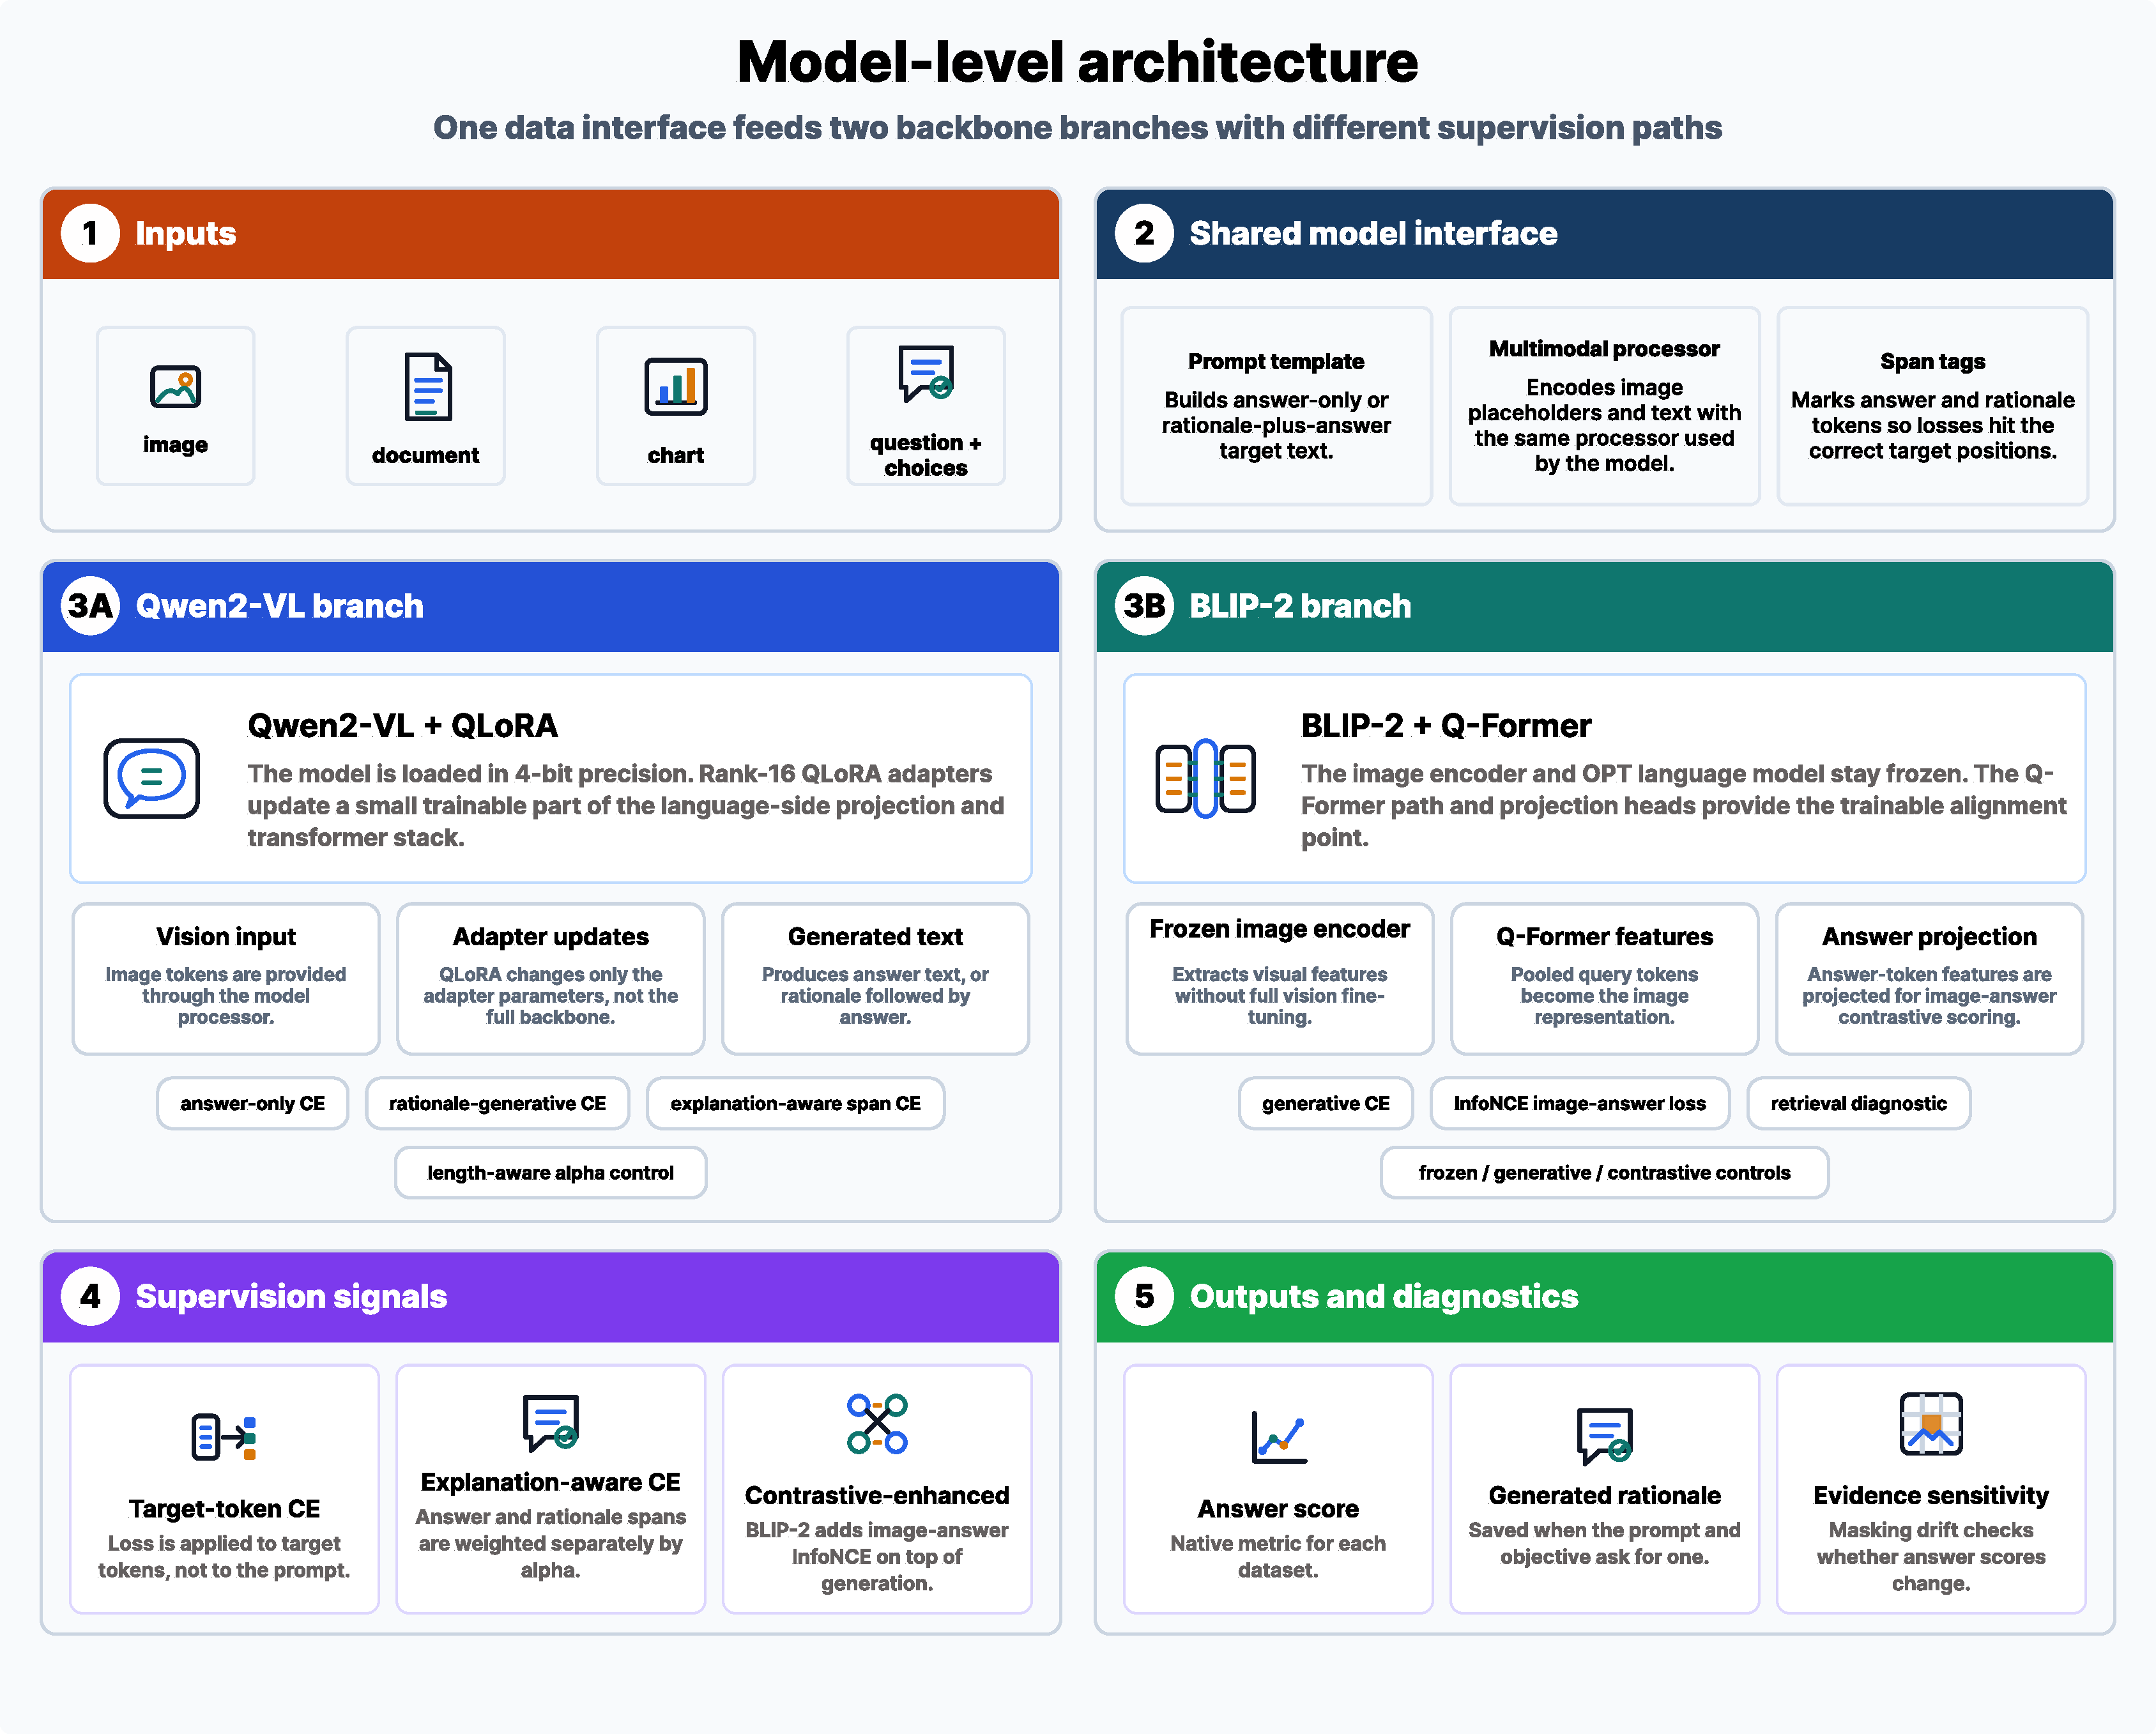
\includegraphics[height=0.74\textheight,keepaspectratio]{./Figures/icons/ModelArchitecture.pdf}}
\caption{Model-level architecture of the controlled alignment setup.
A shared multimodal interface prepares prompts, processor inputs, and supervised spans before routing the run through the Qwen2-VL QLoRA branch or the BLIP-2 Q-Former branch.
Qwen2-VL is used for answer-only, rationale-generative, and explanation-aware supervision, while BLIP-2 is used for generative and contrastive-enhanced controls.}
\label{Fig:Architecture}
\end{figure*}

\begin{equation}
    \mathcal{L} = \alpha\,\mathcal{L}_{\text{answer}} + (1-\alpha)\,\mathcal{L}_{\text{explanation}}
    \label{Eq:Loss}
\end{equation}

Here, $\mathcal{L}_{\text{answer}}$ is the masked cross-entropy loss on the answer tokens, and $\mathcal{L}_{\text{explanation}}$ is the same loss on the explanation tokens.
The coefficient $\alpha$ controls the relative weight of the answer and explanation supervision.

We use two ways of setting $\alpha$.
In fixed-alpha mode, $\alpha$ is chosen explicitly in the experiment configuration serving as an ablation control.
In length-aware mode, the effective answer weight is computed from the number of supervised answer and explanation tokens, as shown in Equation~\ref{Eq:LengthAlpha}:

\begin{equation}
    \alpha_{\text{eff}} =
    \frac{\lambda\,n_{\text{answer}}}{\lambda\,n_{\text{answer}} + n_{\text{explanation}}},
    \label{Eq:LengthAlpha}
\end{equation}
where $n_{\text{answer}}$ and $n_{\text{explanation}}$ are the answer and explanation token counts after collation, and $\lambda$ is the answer-weight multiplier.
When $\lambda=1$, the loss becomes the usual token-level cross-entropy over the full rationale-plus-answer target.
Because of this, the fixed-alpha runs are treated as the ablation, while the length-aware run is used as the natural token-weighted control.

For multiple-choice datasets, inference is done in two steps.
First, a short reasoning sequence is generated given the image and the question.
Then, given that reasoning trace, the model scores each answer option by computing the length-normalised log-likelihood of that option as a continuation of the reasoning.
Afterwards, the option with the highest score is selected as the final answer.
This avoids relying on fragile string parsing or on whether the model copied an option label correctly.
In case of open-ended datasets, the model just generates an answer string, which is evaluated using the dataset's native metric.
When a rationale is generated, it is saved for later use in the rationale quality and evidence sensitivity evaluation.

\section{Evaluation metrics}
Evaluation is divided into three parts: answer quality, rationale quality, and evidence sensitivity.
Answer quality is measured using the native metric of the benchmark, which is the primary metric reported on the leaderboard for that dataset.
We use the term ``headline metric'' to refer to this native primary metric,
not to some universal metric to be compared directly across datasets.
For ScienceQA and A-OKVQA, the headline metric is multiple-choice accuracy.
For DocVQA, it is average normalised Levenshtein similarity (ANLS), as per the benchmark convention~\cite{mathew2021docvqa}.
For ChartQA, it is relaxed accuracy for numerical answers~\cite{masry2022chartqa}.
For the VQAv2 subset, it is VQA consensus accuracy, which is computed wherever annotator answers exist~\cite{antol2015vqa,goyal2017vqav2}.

For rationale quality, we use BLEU and ROUGE-L whenever gold rationales are available~\cite{papineni2002bleu,lin2004rouge}.
These metrics do not measure faithfulness or correctness of the rationale, but they do provide a basic check on 
whether the generated explanation is lexically similar to the gold rationale, and whether it captures the same sequence of reasoning steps.

Evidence sensitivity is measured in an iterative way.
The model's answer is scored on the original image, and then scored again several times by masking out different regions of the image.
This is a general idea of occlusion sensitivity analysis~\cite{zeiler2014visualizing}, adapted to the question-answering setting.
The drift in the answer score when a region is masked out indicates how much the model's answer relies on that region as evidence.
That evidence-masking drift is shown in Equation~\ref{Eq:Drift}.
For qualitative inspection, we compare the regions with high evidence-masking drift to the content named in the generated rationale,
to see if the model is actually naming the evidence it relies on.

\begin{equation}
    \mathrm{drift}(r) = s\!\left(a \mid I\right) - s\!\left(a \mid I \setminus r\right)
    \label{Eq:Drift}
\end{equation}
where $s(a \mid I)$ is the length-normalised log-likelihood of the gold answer $a$ given image $I$, and $I \setminus r$ is the same image with region $r$ occluded.
A large positive drift says the masked region mattered.
A drift near zero says the opposite: the answer probably leaned on language priors, a shortcut, or non-visual context.
The absolute scale does not travel across datasets, since answer length, prompt family, image resolution, and task format all bend the likelihood scores.
The split it captures is the familiar one between a useful explanation and a faithful one.
It also speaks to recent hallucination and critique work, where a model happily describes or relies on visual content that simply is not there~\cite{guan2024hallusionbench,jiang2024hacl,wu2025visco,zhang2025criticv}.
That is why evidence sensitivity sits next to answer accuracy here, rather than being parked as a post-hoc example.

\section{Experimental settings and software used}

Fixed-budget protocol is applied for all the experiments, 
where every run is capped to the same number of training examples,
the same number of evaluation examples, and the same number of seeds.
For Qwen2-VL, the default setup is AdamW optimizer with a learning rate of $2 \times 10^{-4}$,
cosine decay, three percent warm-up, weight decay of 0.01, bf16 compute, and an effective batch size of 32 through gradient accumulation.
The base model is loaded with 4-bit NormalFloat (NF4) quantisation.
QLoRA adapters use rank 16 and scaling factor 32~\cite{hu2022lora,dettmers2023qlora}.
Qwen2-VL-2B-Instruct is the main backbone because it is strong enough while still being small enough to fit the available budget~\cite{wang2024qwen2vl}.
The BLIP-2 experiments use Salesforce BLIP-2 OPT-2.7B, where only Q-Former-side components are trainable, while the vision tower and the OPT language model are frozen~\cite{li2023blip2}.
Qwen2-VL-7B with the same QLoRA setting is used for the scale test.

The split, filtered example count, seed, objective, adapter configuration, and evaluation metrics are recorded for each run.
A split-and-leakage audit is performed for every run, to check the overlap between the train and evaluation identifiers.
The overlap between train and evaluation in the final artifact is zero.
The only non-standard split is DocVQA.
The loaded source provides only validation and test.
That is why the experiment run uses \texttt{validation[:80\%]} for training and \texttt{validation[80\%:]} for evaluation, with native-ID overlap checking.
That audit shows zero native-ID overlap, but it does not guarantee that the train and evaluation sets are completely disjoint in terms of visual content, because the dataset contains multiple questions per document.
For that reason, the DocVQA score is viewed as an internal adaptation result, not as a benchmark claim.

Approximate uncertainty estimates are reported for the accuracy-style headline metrics.
Since most evaluation sets are 200 examples and only a small number of seeds fit the budget,
very small gaps like 0.790 versus 0.795 are treated as observed differences rather than statistically significant ones.
Table~\ref{tab:Config} gives the default configuration used for the Qwen2-VL runs.

\begin{table}[!ht]
\centering
\caption{Default Qwen2-VL QLoRA fine-tuning configuration. BLIP-2 contrastive runs use the separately reported frozen-vision/frozen-LLM Q-Former training setup. Any run that changes these values is reported separately in the experiment ledger and in the Results section.}
\label{tab:Config}
\begin{tabular}{|l|c|}
\hline
\multicolumn{2}{|c|}{\textbf{Training Configuration}} \\ \hline
Adapter & QLoRA (4-bit NF4, rank 16, scaling 32) \\
Optimizer & AdamW ($\beta_1$=0.9, $\beta_2$=0.999) \\
Learning rate & $2 \times 10^{-4}$ (cosine, 3\% warm-up) \\
Weight decay & 0.01 \\
Effective batch size & 32 with gradient accumulation \\
Precision & bf16 compute \\
Primary seed policy & one seed per complete configuration \\ \hline
\end{tabular}
\end{table}

\section{Experiment ledger}
Before reporting the results, a summary of what each group of runs is meant to test is shown in Table~\ref{tab:ExperimentLedger}.
The key boundary is availability of gold rationales.
ScienceQA and A-OKVQA have gold rationales, meaning they support rationale-generative and explanation-aware supervision.
On the other hand, ChartQA, DocVQA, and VQAv2 do not provide the rationale target, so they are considered as answer-only fallback runs for the domain and transfer analyses.

\begin{table*}[!ht]
\centering
\caption{Main experiment ledger. The full generated ledger includes exact caps, seeds, prompt variants, alpha mode, and configuration hashes.}
\label{tab:ExperimentLedger}
\small
\renewcommand{\arraystretch}{1.15}
\begin{tabular}{|>{\raggedright\arraybackslash}p{0.20\textwidth}|>{\raggedright\arraybackslash}p{0.36\textwidth}|>{\raggedright\arraybackslash}p{0.34\textwidth}|}
\hline
\textbf{Comparison} & \textbf{Runs included} & \textbf{Use in the paper} \\ \hline
BLIP-2 objective pair & BLIP-2 OPT-2.7B on ScienceQA: generative and generative+contrastive. & Tests whether the auxiliary contrastive objective contributes anything beyond BLIP-2 generative fine-tuning. \\
ScienceQA controls & Qwen2-VL-2B on ScienceQA: answer-only, rationale+answer CE, fixed-$\alpha$ explanation-aware sweep, and length-aware control. & Separates answer supervision, rationale supervision, and alpha weighting on a gold-rationale dataset. \\
A-OKVQA controls & Qwen2-VL-2B on A-OKVQA: answer-only, rationale+answer CE, fixed-$\alpha$ explanation-aware, and length-aware control. & Repeats the rationale-supervision comparison on a second gold-rationale domain. \\
Fallback domains & Qwen2-VL-2B on ChartQA, DocVQA, and VQAv2 with answer-only fallback prompts. & Reports in-domain adaptation and transfer for datasets without gold rationales; these rows are not used as explanation-aware evidence. \\
Scale & Qwen2-VL-2B and Qwen2-VL-7B on ScienceQA with the same fixed explanation-aware QLoRA setting. & Checks whether the selected setup changes when the backbone scale increases. \\
Transfer & Qwen2-VL-2B source adapters evaluated on target-domain prompts across all datasets. & Tests cross-domain behaviour separately from the official in-domain result table. \\
Masking & Selected Qwen2-VL runs with image-region perturbation and saved visual examples. & Measures evidence sensitivity beside answer accuracy and rationale quality. \\ \hline
\end{tabular}
\end{table*}

\FloatBarrier

    \chapter{Experiments and Results}
The results are reported following the same order as shown in the experiment ledger.
First, the BLIP-2 pair, which tests whether the auxiliary contrastive term adds anything on top of generative fine-tuning.
Then, ScienceQA and A-OKVQA controls, which separate answer-only, rationale-generative, and explanation-aware supervision.
And finally, the last three controls report masking-based visual sensitivity, the Qwen2-VL scale check, and cross-domain transfer.
It is important to note that the results should be viewed in the context of the small-budget protocol, not the leaderboard submissions.

\section{Objective-level comparison}
The objective-level results are shown in Table~\ref{tab:objective_comparison}.
For BLIP-2 on ScienceQA, both objectives yield a slight improvement over the frozen baseline of 0.445.
The contrastive-enhanced run reaches 0.480, while the generative control reaches 0.475.
But the difference is very small and falls within the range of the approximate uncertainty intervals in Table~\ref{tab:uncertainty}.
The same is true for the retrieval diagnostic, where the contrastive-enhanced model has R@1 of 0.010, R@5 of 0.020, R@10 of 0.030, and MRR of 0.0307, which is not a meaningful improvement over the generative control.
Figures~\ref{Fig:BlipObjective} and~\ref{Fig:ContrastiveRetrieval} show these BLIP-2 results.

Qwen2-VL-2B shows stronger results overall.
Rationale-generative fine-tuning scores 0.780 on ScienceQA and 0.790 on A-OKVQA.
Explanation-aware run on A-OKVQA scores 0.795 accuracy, 0.337 ROUGE-L, and 0.087 BLEU.
That is slightly above the generative control, but the difference is small enough that it should be treated as an observed single-run result, not a proven advantage.
The answer-only controls are also strong: 0.800 on ScienceQA and 0.830 on A-OKVQA.
The zero-shot column is reported as a common reference for each model and dataset, not as a separate zero-shot run for every prompt style.
On ScienceQA, the fixed $\alpha=0.50$ explanation-aware run scores 0.765, while the length-aware control scores 0.780, matching the rationale-generative control but still below the answer-only run.
Figure~\ref{Fig:ObjectiveComparison} shows the same controlled comparison visually.

\begin{table*}[!ht]
\centering
\caption{Objective-level results under the controlled protocol. The zero-shot reference is the shared score for the same model and dataset group before the fine-tuning, not a separately recomputed frozen score for every prompt family. Accuracy is multiple-choice accuracy for ScienceQA and A-OKVQA.}
\label{tab:objective_comparison}
\scriptsize
\begin{adjustbox}{max width=\textwidth}
\begin{tabular}{|l|l|l|c|c|c|c|}
\hline
\textbf{Backbone} & \textbf{Dataset} & \textbf{Objective} & \textbf{Zero-shot ref.} & \textbf{Final} & \textbf{ROUGE-L} & \textbf{BLEU} \\ \hline
BLIP-2 OPT-2.7B & ScienceQA & Generative & 0.445 & 0.475 & -- & -- \\
BLIP-2 OPT-2.7B & ScienceQA & Contrastive-enhanced & 0.445 & 0.480 & -- & -- \\
Qwen2-VL-2B & ScienceQA & Answer-only & 0.400 & \textbf{0.800} & -- & -- \\
Qwen2-VL-2B & ScienceQA & Rationale+answer CE & 0.400 & 0.780 & 0.693 & 0.559 \\
Qwen2-VL-2B & ScienceQA & Explanation-aware, $\alpha=0.50$ & 0.400 & 0.765 & 0.643 & 0.493 \\
Qwen2-VL-2B & ScienceQA & Explanation-aware, length-aware & 0.400 & 0.780 & 0.696 & 0.563 \\
Qwen2-VL-2B & A-OKVQA & Answer-only & 0.355 & \textbf{0.830} & -- & -- \\
Qwen2-VL-2B & A-OKVQA & Rationale+answer CE & 0.355 & 0.790 & 0.329 & 0.083 \\
Qwen2-VL-2B & A-OKVQA & Explanation-aware, $\alpha=0.50$ & 0.355 & 0.795 & 0.337 & 0.087 \\
Qwen2-VL-2B & A-OKVQA & Explanation-aware, length-aware & 0.355 & 0.790 & 0.330 & 0.083 \\ \hline
\end{tabular}
\end{adjustbox}
\end{table*}

\begin{table*}[!ht]
\centering
\caption{Approximate uncertainty for selected accuracy-style headline metrics. These intervals use the generated normal-approximation standard errors for capped evaluation sets, so they are a caution about small observed differences rather than a replacement for multi-seed testing.}
\label{tab:uncertainty}
\scriptsize
\begin{adjustbox}{max width=\textwidth}
\begin{tabular}{|l|l|c|c|c|}
\hline
\textbf{Run} & \textbf{Metric} & \textbf{Eval cap} & \textbf{Score} & \textbf{Approx. 95\% CI} \\ \hline
BLIP-2 generative ScienceQA & MC accuracy & 200 & 0.475 & 0.406--0.544 \\
BLIP-2 contrastive ScienceQA & MC accuracy & 200 & 0.480 & 0.411--0.549 \\
ScienceQA answer-only & MC accuracy & 200 & 0.800 & 0.745--0.855 \\
ScienceQA rationale+answer CE & MC accuracy & 200 & 0.780 & 0.723--0.837 \\
ScienceQA explanation-aware, $\alpha=0.50$ & MC accuracy & 200 & 0.765 & 0.706--0.824 \\
ScienceQA explanation-aware, length-aware & MC accuracy & 200 & 0.780 & 0.723--0.837 \\
A-OKVQA answer-only & MC accuracy & 200 & 0.830 & 0.778--0.882 \\
A-OKVQA rationale+answer CE & MC accuracy & 200 & 0.790 & 0.734--0.847 \\
A-OKVQA explanation-aware, $\alpha=0.50$ & MC accuracy & 200 & 0.795 & 0.739--0.851 \\
Qwen2-VL-7B ScienceQA, $\alpha=0.50$ & MC accuracy & 200 & 0.885 & 0.841--0.929 \\ \hline
\end{tabular}
\end{adjustbox}
\end{table*}

\begin{figure}[!ht]
\centerline{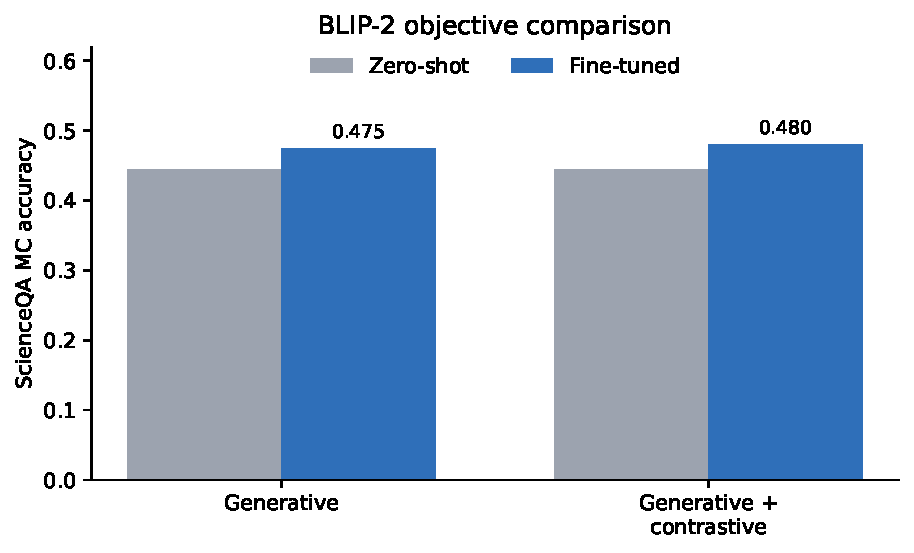
\includegraphics[width=0.82\linewidth]{./Figures/generated/blip2_objective}}
\caption{BLIP-2 generative and contrastive-enhanced ScienceQA results.
Both runs improve over the frozen baseline, with only a small observed gain from the auxiliary contrastive term.}
\label{Fig:BlipObjective}
\end{figure}

\begin{figure}[!ht]
\centerline{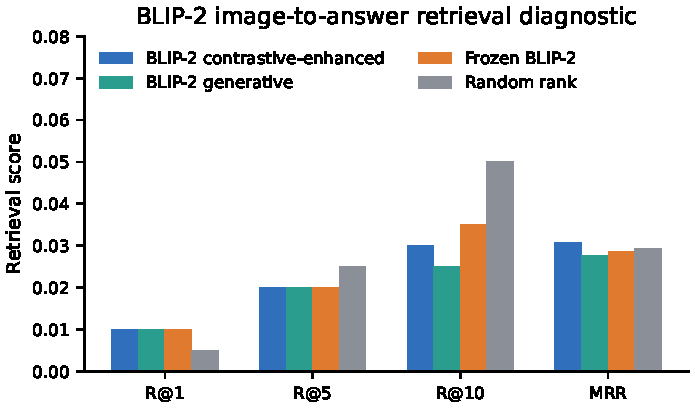
\includegraphics[width=0.82\linewidth]{./Figures/generated/contrastive_retrieval}}
\caption{BLIP-2 image-to-answer retrieval diagnostic.
The analysis reports frozen BLIP-2, BLIP-2 generative, BLIP-2 contrastive-enhanced, and random-rank controls so the contrastive branch is not interpreted without a reference point.}
\label{Fig:ContrastiveRetrieval}
\end{figure}

\begin{figure}[!ht]
\centerline{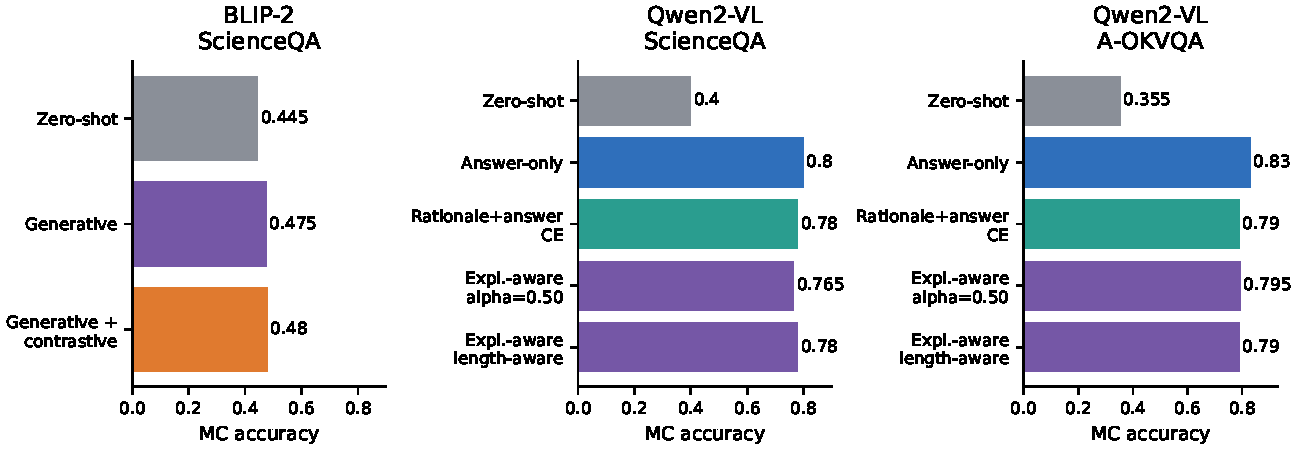
\includegraphics[width=\linewidth]{./Figures/generated/controlled_strategy_comparison}}
\caption{Controlled strategy comparison for BLIP-2 and Qwen2-VL.
The figure shows zero-shot, answer-only, rationale-generative, explanation-aware, and contrastive variants where those controls are available.}
\label{Fig:ObjectiveComparison}
\end{figure}

\FloatBarrier

\section{Effect of explanation-aware training}
Table~\ref{tab:alpha_sweep} and Figure~\ref{Fig:AlphaSweep} show the ScienceQA fixed-$\alpha$ sweep.
Here $\alpha$ is the answer-span weight from Equation~\ref{Eq:Loss}.
Fine-tuning raises accuracy from the 0.400 zero-shot reference into the 0.690--0.780 range.
The best fixed setting is low answer weight: $\alpha=0.10$, which reaches 0.780.
As $\alpha$ moves toward the answer-heavy end, accuracy drops to 0.690 at $\alpha=0.75$ and 0.695 at $\alpha=1.00$.
The same pattern is observed on the rationale metrics.
ROUGE-L and BLEU also reach the maximum at $\alpha=0.10$ (0.695 and 0.566), then decline as $\alpha$ increases.
At $\alpha=1.00$, only the answer span is supervised inside a target but the rationale part is still included in the target template, although it is not weighted in the loss. Hence, the rationale metrics are not computed in that case.

The $\alpha=0.10$ run matches the rationale-generative and length-aware controls on accuracy.
The $\alpha=1.00$ run should not be confused with a true answer-only run, because the target template in that case still contains the rationale part,
even though that rationale span is not included in the loss.
The answer-only control on ScienceQA is trained with a target that contains only the answer part of the template, reaches 0.800,
which is above the best fixed-$\alpha$ run and the rationale-generative control.
All of these comparisons use one seed, 2{,}000 training examples, and 200 evaluation examples, so they show observed behaviour rather than final statistical proof.

\begin{table}[!ht]
\centering
\caption{Explanation-aware fixed-$\alpha$ sweep on ScienceQA (Qwen2-VL-2B, QLoRA, 2{,}000 train / 200 eval, single seed). The coefficient $\alpha$ weights the answer span in Equation~\ref{Eq:Loss}: $\alpha=1$ is answer-span-only within the rationale target and $\alpha=0$ is explanation-span-only. The zero-shot and rationale-generative rows are references. Random-choice accuracy is 0.354. The best fixed $\alpha$ is shown in bold.}
\label{tab:alpha_sweep}
\begin{tabular}{|l|c|c|c|}
\hline
\textbf{Variant ($\alpha$)} & \textbf{MC accuracy} & \textbf{ROUGE-L} & \textbf{BLEU} \\ \hline
Zero-shot (frozen) & 0.400 & -- & -- \\
Rationale+answer CE & \textbf{0.780} & 0.693 & 0.559 \\ \hline
$\alpha=0.00$ (explanation-only) & 0.725 & 0.417 & 0.299 \\
$\alpha=0.10$ & \textbf{0.780} & \textbf{0.695} & \textbf{0.566} \\
$\alpha=0.25$ & 0.775 & 0.686 & 0.548 \\
$\alpha=0.50$ & 0.765 & 0.643 & 0.493 \\
$\alpha=0.75$ & 0.690 & 0.604 & 0.443 \\
$\alpha=1.00$ (answer-span only) & 0.695 & -- & -- \\ \hline
\end{tabular}
\end{table}

\begin{figure}[!ht]
\centerline{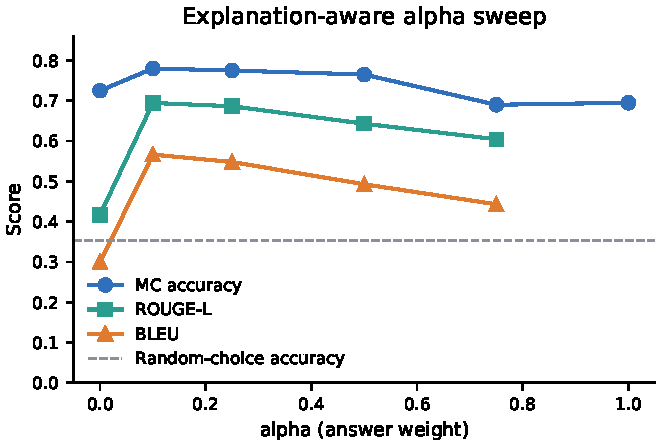
\includegraphics[width=0.82\linewidth]{./Figures/generated/alpha_sweep}}
\caption{Fixed-alpha explanation-aware sweep on ScienceQA.
Answer accuracy peaks at the low-answer-weight setting and declines toward both extremes inside the rationale-plus-answer target.
Explanation quality (ROUGE-L, BLEU) peaks at the same point and falls as $\alpha$ increases.
Series are distinguished by marker shape and line style; the dashed grey line marks random-choice accuracy. Single seed.}
\label{Fig:AlphaSweep}
\end{figure}

\FloatBarrier

\section{Domain-level behaviour}
Table~\ref{tab:domain_results} and Figure~\ref{Fig:CrossDomain} represent the results for the selected in-domain runs.
Fixed $\alpha=0.50$ is used for the ScienceQA row, so that it matches the selected domain comparison.
The stronger $\alpha=0.10$ and length-aware settings are reported separately in the sweep above.
A-OKVQA rises from 0.355 to 0.795 accuracy against the zero-shot reference.
The VQAv2 subset rises from 0.350 to 0.730 VQA accuracy.
ChartQA reaches 0.655 relaxed accuracy, with exact match at 0.410.
DocVQA reaches 0.905 ANLS and 0.855 exact match.
Although the DocVQA score is strong in this run, it should be read carefully, because the examples are mostly short extractive answers, the training setup is answer-only fallback rather than gold-rationale supervision, and the split audit cannot prove document-level disjointness beyond the native IDs exposed by the loader.

\begin{table*}[!ht]
\centering
\caption{Domain-level results for the completed Qwen2-VL-2B runs. Each domain uses its native headline metric: multiple-choice accuracy for ScienceQA and A-OKVQA, relaxed accuracy for ChartQA, ANLS for DocVQA, and VQA accuracy for the VQAv2 subset.}
\label{tab:domain_results}
\scriptsize
\begin{adjustbox}{max width=\textwidth}
\begin{tabular}{|l|l|l|c|c|c|}
\hline
\textbf{Domain} & \textbf{Dataset} & \textbf{Objective} & \textbf{Zero-shot ref.} & \textbf{Final} & \textbf{Secondary metric} \\ \hline
Science & ScienceQA & Explanation-aware, $\alpha=0.50$ & 0.400 & 0.765 & ROUGE-L 0.643, BLEU 0.493 \\
Commonsense & A-OKVQA & Explanation-aware, $\alpha=0.50$ & 0.355 & 0.795 & ROUGE-L 0.337, BLEU 0.087 \\
Charts & ChartQA & Answer-only fallback & 0.335 & 0.655 & Exact match 0.410 \\
Documents & DocVQA & Answer-only fallback & 0.349 & 0.905 & Exact match 0.855 \\
Natural images & VQAv2 subset & Answer-only fallback & 0.350 & 0.730 & Exact match 0.350 $\rightarrow$ 0.730 \\ \hline
\end{tabular}
\end{adjustbox}
\end{table*}

\begin{figure}[!ht]
\centerline{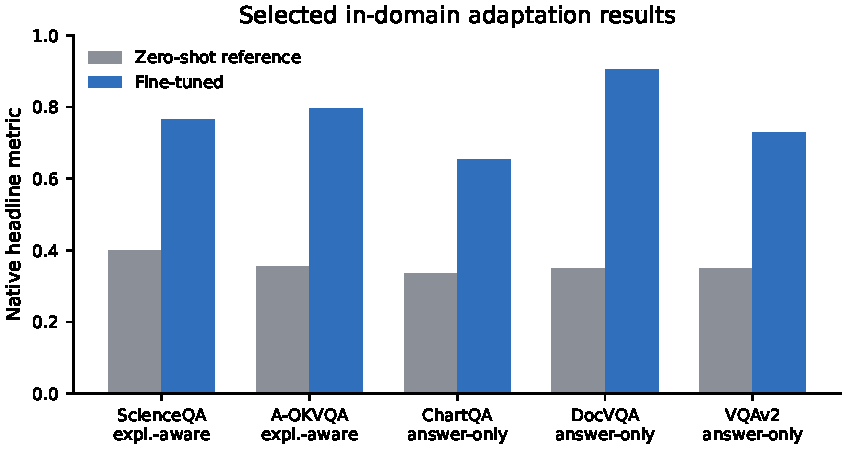
\includegraphics[width=0.82\linewidth]{./Figures/generated/cross_domain}}
\caption{In-domain adaptation results for the selected completed Qwen2-VL-2B domain runs.
The comparison mixes rationale-supervised ScienceQA/A-OKVQA rows with answer-only fallback rows for domains without gold rationales, so it should not be read as an explanation-aware effect across all domains.}
\label{Fig:CrossDomain}
\end{figure}

\FloatBarrier

\section{Faithfulness and hallucination analysis}
Evidence-masking drift is shown in Table~\ref{tab:faithfulness} and Figure~\ref{Fig:Faithfulness}.
Each value is averaged over 30 evaluation examples.
Higher positive drift means that the model produced lower probability for the real answer when the masked region was occluded, meaning that the model relied on that region as evidence for the answer.
The strongest evidence sensitivity is observed in the structured tasks: DocVQA at 0.375, ChartQA at 0.224, and VQAv2 at 0.111.
ScienceQA and A-OKVQA are much lower, with the ScienceQA answer-only adapter as the main exception at 0.0898.

Low ScienceQA drift is understandable, because many ScienceQA items could be partly answered based on the question and the answer choices using the learned facts, the relevant visual evidence can be spread across the image, and a coarse mask may miss the regions the model actually uses.
Explanation supervision does not create a clean drift pattern in this run.
The $\alpha=0.10$ setting gives 0.0223, $\alpha=0.50$ gives 0.0197, and answer-span-only $\alpha=1.00$ gives 0.0149, even though that run has no supervised rationale metric.
On A-OKVQA, the explanation-aware run has slightly higher drift than the generative control (0.0271 versus 0.0245), but both intervals are wide.
Hence, the evidence-masking results do not demonstrate that the explanation-aware training yields a stronger visual sensitivity than the rationale-generative control.
Figure~\ref{Fig:MaskingExample} shows one saved masking example.

\begin{table}[!ht]
\centering
\caption{Evidence-masking drift by completed run. Higher values indicate stronger sensitivity to masked visual evidence. The intervals are approximate 95\% intervals from the generated masking artifact.}
\label{tab:faithfulness}
\scriptsize
\begin{adjustbox}{max width=\textwidth}
\begin{tabular}{|l|c|c|c|}
\hline
\textbf{Run} & \textbf{Mean drift} & \textbf{Approx. 95\% CI} & \textbf{Examples} \\ \hline
ScienceQA answer-only & 0.0898 & 0.0197--0.1830 & 30 \\
ScienceQA rationale+answer CE & 0.0217 & -0.0100--0.0582 & 30 \\
ScienceQA $\alpha=0.10$ & 0.0223 & -0.0080--0.0568 & 30 \\
ScienceQA $\alpha=0.50$ & 0.0197 & -0.0119--0.0552 & 30 \\
ScienceQA answer-span-only $\alpha=1.00$ & 0.0149 & -0.0274--0.0638 & 30 \\
A-OKVQA rationale+answer CE & 0.0245 & -0.0236--0.0726 & 30 \\
A-OKVQA explanation-aware & 0.0271 & -0.0075--0.0627 & 30 \\
ChartQA answer-only fallback & 0.2237 & 0.1419--0.3140 & 30 \\
DocVQA answer-only fallback & 0.3749 & 0.2770--0.4960 & 30 \\
VQAv2 answer-only fallback & 0.1109 & 0.0274--0.2408 & 30 \\
Qwen2-VL-7B ScienceQA $\alpha=0.50$ & 0.0114 & -0.0059--0.0260 & 30 \\ \hline
\end{tabular}
\end{adjustbox}
\end{table}

\begin{figure}[!ht]
\centerline{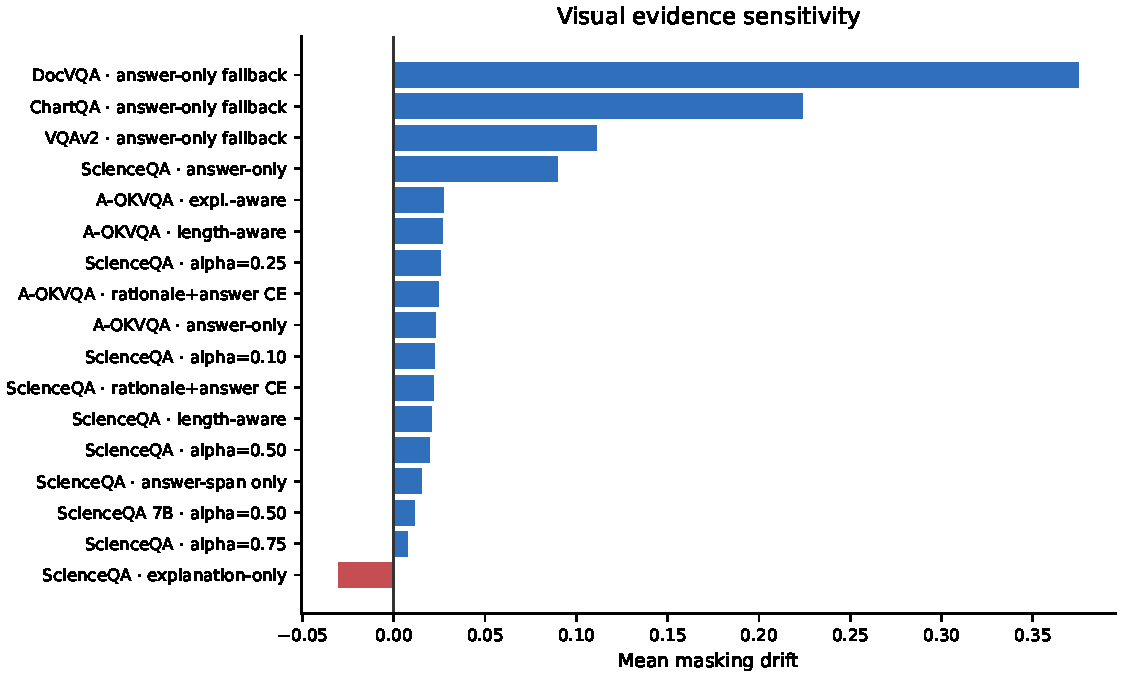
\includegraphics[width=0.82\linewidth]{./Figures/generated/faithfulness}}
\caption{Mean evidence-masking drift across completed runs.
Structured document and chart runs show much stronger visual sensitivity than the rationale-rich ScienceQA and A-OKVQA runs, but stronger drift does not automatically imply better answer accuracy.}
\label{Fig:Faithfulness}
\end{figure}

\IfFileExists{./Figures/generated/masking_example_chartqa_clean.pdf}{
\begin{figure*}[!ht]
\centerline{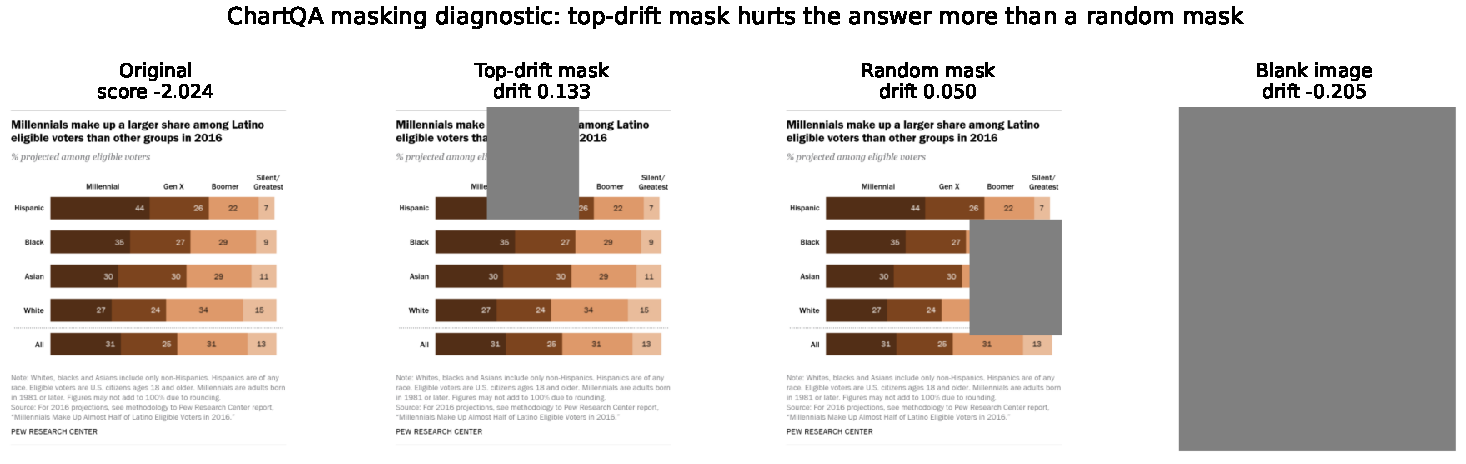
\includegraphics[width=\linewidth]{./Figures/generated/masking_example_chartqa_clean}}
\caption{Example masking diagnostic for a ChartQA answer-only fallback run.
The pipeline saves the original image, the top-drift mask, a random-region mask, and a blank-image control, together with the full-image and masked answer scores.
This figure is used as an evidence-sensitivity example, not as proof that a generated rationale is faithful.}
\label{Fig:MaskingExample}
\end{figure*}
}{}

\FloatBarrier

\section{Efficiency and scale trade-offs}
The comparison between Qwen2-VL-2B and Qwen2-VL-7B using the same ScienceQA explanation-aware setting ($\alpha=0.50$) is shown in Table~\ref{tab:scale} and Figure~\ref{Fig:Scale}.
The larger model shows a clear improvement in the completed experiments.
Accuracy rises from 0.765 to 0.885.
ROUGE-L moves from 0.643 to 0.738, and BLEU moves from 0.493 to 0.637.
The comparison is still within the same parameter-efficient setting, because both runs are fine-tuned using the same QLoRA setup.
However, the logs do not include the exact GPU hours or memory usage for each run, so we treat this as a scale comparison rather than a full efficiency benchmark.

\begin{table}[!ht]
\centering
\caption{Qwen2-VL scale comparison on ScienceQA with the same explanation-aware objective ($\alpha=0.50$).}
\label{tab:scale}
\begin{tabular}{|l|c|c|c|}
\hline
\textbf{Model} & \textbf{MC accuracy} & \textbf{ROUGE-L} & \textbf{BLEU} \\ \hline
Qwen2-VL-2B & 0.765 & 0.643 & 0.493 \\
Qwen2-VL-7B & \textbf{0.885} & \textbf{0.738} & \textbf{0.637} \\ \hline
\end{tabular}
\end{table}

\begin{figure}[!ht]
\centerline{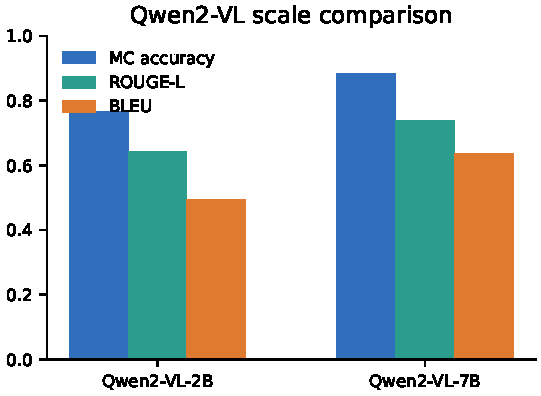
\includegraphics[width=0.82\linewidth]{./Figures/generated/scale_comparison}}
\caption{Scale comparison for the fixed ScienceQA explanation-aware setting.
Moving from Qwen2-VL-2B to Qwen2-VL-7B improves both answer accuracy and rationale-overlap metrics.}
\label{Fig:Scale}
\end{figure}

\FloatBarrier

\section{Cross-domain transfer}
Table~\ref{tab:transfer} and Figure~\ref{Fig:Transfer} present the transfer matrix from training domain to evaluation domain.
Each column uses the metric of the target dataset, so values should be compared within a column rather than across a row.
The matrix keeps answer-only, rationale-generative, and explanation-aware sources separate.
This table is a transfer probe, not a replacement for the in-domain results.
Since the transfer evaluator might use a different prompt family than the in-domain evaluation (e.g., answer-only transfer evaluated with an answer-only prompt), the diagonal values may not be exactly the same as the in-domain table.

The transfer results are not explained by the dataset domain alone, meaning that the training objective also influences how well a model transfers.
The ScienceQA answer-only adapter transfers well, reaching 0.805 on A-OKVQA, 0.645 on ChartQA, 0.703 on DocVQA, and 0.630 on VQAv2.
The ScienceQA rationale-generative and explanation-aware adapters are above random baselines, but they transfer less well to ChartQA, DocVQA, and VQAv2 compared to the answer-only adapter.
For A-OKVQA sources, rationale-generative training gives the strongest DocVQA transfer in that group (0.764), while answer-only training gives the strongest VQAv2 transfer (0.700).
DocVQA is strongest in-domain at 0.910, and the document-trained adapter also transfers well to ChartQA at 0.685.
Overall, transfer depends on both the target domain and the source objective.

\begin{table*}[!ht]
\centering
\caption{Cross-domain transfer matrix. Rows indicate the training domain and columns indicate the evaluation domain. Each column uses the target domain's headline metric, so values are best compared within a column.}
\label{tab:transfer}
\scriptsize
\begin{adjustbox}{max width=\textwidth}
\begin{tabular}{|l|ccccc|}
\hline
\textbf{Trained on} & \textbf{ScienceQA} & \textbf{A-OKVQA} & \textbf{ChartQA} & \textbf{DocVQA} & \textbf{VQAv2} \\ \hline
ScienceQA answer-only & 0.800 & 0.805 & 0.645 & 0.703 & 0.630 \\
ScienceQA rationale CE & 0.780 & 0.760 & 0.450 & 0.559 & 0.300 \\
ScienceQA explanation-aware & 0.740 & 0.765 & 0.460 & 0.491 & 0.410 \\
A-OKVQA answer-only & 0.690 & 0.825 & 0.635 & 0.677 & 0.700 \\
A-OKVQA rationale CE & 0.665 & 0.790 & 0.645 & 0.764 & 0.600 \\
A-OKVQA explanation-aware & 0.680 & 0.795 & 0.615 & 0.763 & 0.640 \\
ChartQA answer-only & 0.420 & 0.415 & 0.660 & 0.831 & 0.680 \\
DocVQA answer-only & 0.450 & 0.435 & 0.685 & 0.910 & 0.660 \\
VQAv2 answer-only & 0.440 & 0.575 & 0.660 & 0.716 & 0.730 \\ \hline
\end{tabular}
\end{adjustbox}
\end{table*}

\begin{figure}[!ht]
\centerline{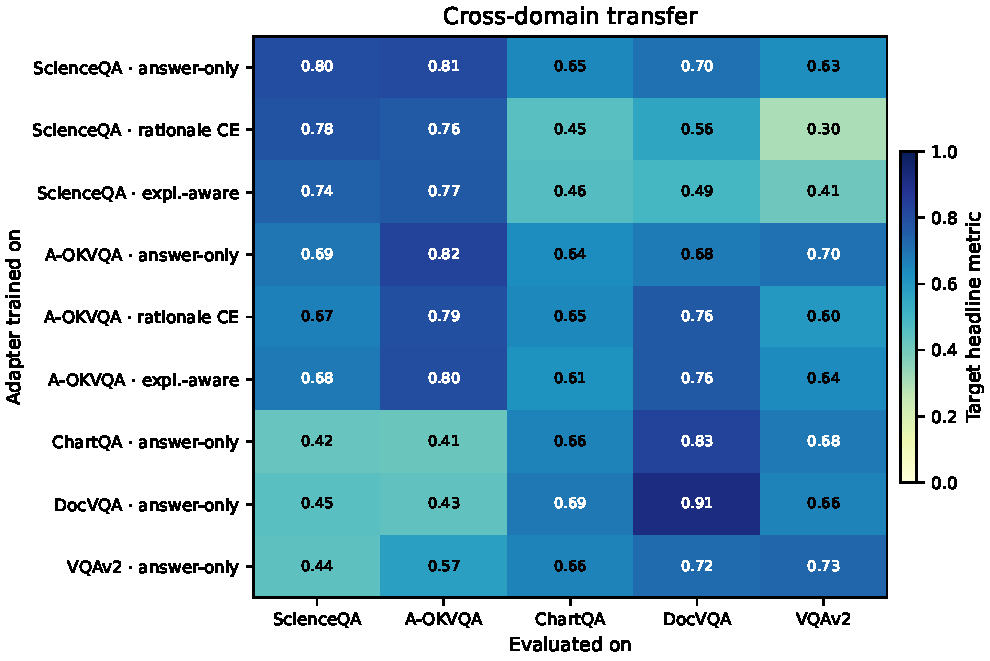
\includegraphics[width=0.76\linewidth]{./Figures/generated/transfer_matrix}}
\caption{Cross-domain transfer heatmap.
The strongest non-diagonal transfer is not always from the visually closest domain.
Answer-only ScienceQA transfers strongly to A-OKVQA, while answer-only document and chart adapters transfer strongly to several open-ended targets.}
\label{Fig:Transfer}
\end{figure}

\FloatBarrier

    \chapter{Conclusion}
\section{Discussion}
The results do support the main idea in some ways, but not as a simple success story.
Changing the objective does change the behaviour of the model,
but the claim that explanation supervision is always better than answer-only supervision is clearly not supported by the results of the completed runs.
Answer-only training is the strongest on both ScienceQA and A-OKVQA.
On ScienceQA, the best fixed explanation-aware run is achieved when the answer weight is low ($\alpha=0.10$), and the length-aware control is close to the rationale-generative control, while the answer-span-only control performs worse than both of those.
The same story can be seen on A-OKVQA, where explanation-aware training improves the accuracy above the rationale-generative control,
but the gap is small enough that it should not be treated as statistically significant given the capped evaluation protocol.

The fixed $\alpha=0.50$ ScienceQA run is also below the rationale-generative and answer-only controls.
So the main takeaway is not just ``add explanations'', but rather find the right balance of answer and rationale supervision for the domain and model.

The BLIP-2 contrastive result is also modest.
On ScienceQA, the contrastive-enhanced control improves the performance just slightly above the generative control (0.480 versus 0.475),
but that difference is statistically insignificant given the approximate confidence intervals.
The retrieval diagnostic tells the same story, staying close to the frozen and random references.
In this setup, the auxiliary image--answer InfoNCE term does not produce any stronger representation by itself.
That is still a useful result, because it keeps the contrastive branch from being viewed as helpful just because it adds more seemingly useful signal to the training.

The domain results show why the study needs more than one benchmark.
ScienceQA and A-OKVQA are used for the rationale-supervised training, because they provide the gold explanations that make that training possible.
ChartQA, DocVQA, and VQAv2, on the other hand, do not have gold explanations, and that is why those runs are used only for answer-only adaptation 
and domain transfer testing across structured documents, charts and natural images, rather than for rationale-supervised training.
They are used to show how the same fine-tuning pipeline behaves when moved to domain where the model must answer directly without gold rationale supervision.
For the stronger document-faithfulness claim we would need document-specific rationale labels or a more direct OCR/layout intervention test, because the current setup does not strongly prove that the model is using the document evidence in a faithful way, even though it achieves a strong ANLS score.

The masking results should also be interpreted carefully.
If masking some region causes the answer score to drop, that means that the model is sensitive to that part of the image.
However, that does not automatically mean that the generated explanation is faithful.
DocVQA and ChartQA show higher masking drift because their answers often depend on local text, labels, or layout, even though those runs use answer-only training.
On ScienceQA and A-OKVQA, the masking drift is low and does not change much with the explanation-aware training, even though the rationale metrics do improve.
That shows that the explanation quality and the visual sensitivity are not perfectly correlated.
That is why, masking drift should be considered as an evidence-sensitivity test rather than as a proof of faithful explanation generation.

The cleanest positive result is seen in the scale comparison.
Holding the ScienceQA explanation-aware objective fixed and moving from Qwen2-VL-2B to Qwen2-VL-7B improves accuracy from 0.765 to 0.885, ROUGE-L from 0.643 to 0.738, and BLEU from 0.493 to 0.637.
However, this does not mean that the 2B runs are not useful, because the smaller model makes the broader sweep of configurations affordable.
It does suggest that some of the weaker 2B results are capacity-related rather than only objective-related.

Transfer is mixed too.
Answer-only supervision on ScienceQA transfers well to A-OKVQA, ChartQA, DocVQA, and VQAv2, while rationale-generative and explanation-aware training on ScienceQA perform worse on those targets.
On A-OKVQA however, the rationale-generative and explanation-aware runs transfer better to DocVQA than the answer-only run, while the answer-only run transfers better to VQAv2.
The DocVQA adapter is strong in-domain and also transfers well to ChartQA even though the visual format is quite different, which suggests that the model learns some useful structured, text-heavy visual reading skills that can be carried from documents to charts.
Overall, these results show that the transfer depends on the trained objective and the dataset domain of both source and target.

\section{Limitations}
There are several limitations in this study that should be considered when reading the results and claims.
The first and most important one is the compute.
To keep this study feasible for a small project, all the experiments are run in a single-GPU environment, which consequently limits the number of seeds, model sizes, and full-dataset runs that can be completed.

The second limitation is the rationale availability in the datasets.
ScienceQA and A-OKVQA do provide gold explanations, which enables the rationale-supervised training, while DocVQA, ChartQA, and VQAv2 do not, which is why those datasets are used for answer-only adaptation and transfer testing rather than for rationale-supervised training.

The third limitation is metric quality.
BLEU and ROUGE-L are good for measuring overlap between the generated rationale and the gold rationale, but they can miss valid explanations when the model generates the same meaning with different wording.
Masking drift is close to visual evidence use, but it can be noisy for highly dispersed evidence or dense documents and charts, where the masked region might not actually cover the full region of the evidence the model uses.

The fourth limitation is the capped protocol.
Most runs use limited training and evaluation subsets instead of the full datasets with a single seed for each configuration due to resource constraints.
This makes the work possible. However, it also means that the results should not be viewed as fully representative.
Finally, the execution logs validate the produced outputs, but they are not enough for precise wall-clock or peak-memory benchmarking.

These limitations define how far the claims in this paper should go.

\section{Summary}
This paper studied the effect of training objectives on the behaviour of the model, while keeping other factors such as the model architecture, data setup, and compute budget fixed.
It compared zero-shot references, BLIP-2 generative and contrastive-enhanced supervision, and Qwen2-VL with answer-only, rationale-generative, and explanation-aware training across document, chart, science, commonsense, and natural-image domains.
The evaluation measured answer accuracy, rationale quality where gold rationales are available, and visual sensitivity, instead of looking at final accuracy alone.

The main outcome is that explanation-aware training can improve the quality of the generated rationales, but that does not mean the model performs better in that setting compared to answer-only training, at least not in the completed runs.
It also shows that the ratio of answer supervision to rationale supervision matters, and that the best setting is not necessarily the one with the strongest rationale supervision.
The completed runs also suggest that BLIP-2 contrastive-enhanced training does not contribute much to final accuracy or retrieval performance compared to the generative control.

At the same time, the domain results show that the same pipeline can still be useful outside the rationale-supervised datasets.
ScienceQA and A-OKVQA are the main datasets for testing rationale supervision, while ChartQA, DocVQA, and VQAv2 are used to test answer-only adaptation and transfer across different visual domains.
The selected runs improve on all five datasets, but the meaning of the improvement depends on the type of training used for each dataset.
For example, the DocVQA result shows strong capped document-answering performance, but it does not prove faithful document explanation generation.

The faithfulness analysis also needs to be read carefully.
Masking drift shows whether the model is sensitive to visual evidence, but it should not be considered as a full proof that the generated explanation is faithful.
In some settings, the model can generate better rationales without showing a clear increase in masking-based visual sensitivity.
This means that good explanation text is not fully correlated with the actual use of visual evidence.

The scale comparison gives the clearest positive result.
When the same ScienceQA explanation-aware setup is moved from Qwen2-VL-2B to Qwen2-VL-7B, the larger model improves both answer accuracy and rationale metrics.
The transfer results are more mixed, showing that a fine-tuned adapter does not transfer equally well to every target domain.
Overall, the study shows that supervised rationales can be useful for low-resource VLM fine-tuning, but their value is only clear when they are compared with answer-only training and tested for domain transfer and visual evidence sensitivity.

\section{Outlook}
The first future direction would be to increase the number of seeds and the dataset size for the strongest configurations.
A second step would be to test more recent open multimodal backbones, while keeping the same objective-isolation protocol.
Another direction is to add rationale annotation for document and chart datasets, because faithful explanations in those domains would be very valuable.
Also, more causal masking tests would be useful.
Future work could apply edits to the document text, chart labels, or some regions of the image in a controlled way, instead of only masking, and measure how the answer changes after those edits.
Additionally, it would be interesting to compare supervised explanation-aware training with reinforcement learning or preference-based methods where the model is rewarded for grounded reasoning directly.
Measuring latency, memory, and calibration together with accuracy and faithfulness would also be important for practical deployment, especially as the model size increases.

% ---------------------------------------------------------------


% ---------------------------------------------------------------
\backmatter % no page numbering from here
    \newacronym{vlm}{VLM}{vision--language model}
\newacronym{vqa}{VQA}{visual question answering}
\newacronym{qlora}{QLoRA}{quantised low-rank adaptation}
\newacronym{lora}{LoRA}{low-rank adaptation}
\newacronym{blip}{BLIP-2}{Bootstrapping Language-Image Pre-training, version 2}
\newacronym{anls}{ANLS}{average normalised Levenshtein similarity}
\glsaddall

    \newglossaryentry{crossmodalalignment}{name={cross-modal alignment},description={The process of connecting visual and language signals so that a model can use both in one task}}
\newglossaryentry{evidencesensitivity}{name={evidence sensitivity},description={A diagnostic showing whether the model score changes when visually relevant image regions are perturbed}}
\newglossaryentry{rationale}{name={rationale},description={A generated explanation that connects the question, visual input, and final answer}}
\glsaddall

    % \clearpage
    \printglossary[title={Acronyms}, type=\acronymtype, toctitle=List of Acronyms]
    \printglossary[title=Special Terms, toctitle=List of terms]

		% if you want to provide a glossary with explanations of important terms put it in here

    \nocite{radford2021clip,jia2021align,li2022blip,alayrac2022flamingo,liu2023llava,zhu2023minigpt4,dai2023instructblip,wang2022ofa,wang2022git,bai2023qwenvl,chen2023pali,awadalla2023openflamingo,agrawal2017vqa,marino2019okvqa,singh2019textvqa,hudson2019gqa,johnson2017clevr,kafle2018dvqa,kahou2018figureqa,kim2020plotqa,mathew2022infographicvqa,mishra2019ocrvqa,houlsby2019adapters,li2021prefix,lester2021prompt,liu2022ptuningv2,zaken2022bitfit,sung2022vladapter,selvaraju2017gradcam,ribeiro2016lime,sundararajan2017axiomatic,chefer2021transformer,li2023pope,fu2023mme,liu2023mmbench,li2024seedbench,yu2024mmvet,zhang2020bertscore,banerjee2005meteor,sellam2020bleurt,krishna2017visualgenome,plummer2015flickr30k,kazemzadeh2014referitgame,yu2016modelingvisual,wang2024cogvlm}
    \bibliographystyle{geralpha}
    \bibliography{./bib/manual}

    \chapter*{Declarations}
    \addcontentsline{toc}{chapter}{Declarations}
\textbf{Author responsibility.}
The authors wrote, reviewed, and edited the manuscript and take full responsibility for the final content, results, and claims.

\textbf{Use of generative AI.}
Generative AI tools were used only for language editing, code assistance, and consistency checks.
All scientific decisions, experiment selection, result interpretation, and final manuscript approval remain the responsibility of the authors.

\textbf{Funding.}
No external funding was received for this study.

\textbf{Conflict of interest.}
The authors declare no conflict of interest.

\textbf{Data, code, and artifacts.}
The experiments use public datasets cited in the paper.
The code, configuration files, generated tables, figures, execution logs, and claim-to-evidence artifacts are maintained with the project repository and can be made available with the submitted supplementary material.
The project repository is available at \url{https://github.com/Kamran151199/thesis}.

\chapter*{Annex}
    \addcontentsline{toc}{chapter}{Annex}
    Supplementary artifacts, generated figures, tables, execution logs, and configuration files are maintained with the project repository: \url{https://github.com/Kamran151199/thesis}.


\end{document}
